%%
%%  chapter07.tex - Obstacle Detection and Planning for Autonomous Vehicles based on Computer Vision Techniques
%%
%%  Copyright 2014 Néstor Morales <nestor@isaatc.ull.es>
%%
%%  This work is licensed under a Creative Commons Attribution 4.0 International License.
%%

\graphicspath{{./images/chapter07/bmps/}{./images/chapter07/vects/}{./images/chapter07/}}

\chapter{Local Planning}\label{ch:chapter07}

By using the methods described in previous chapters, the vehicle is able to detect the obstacles in the surrounding area, and knows how to reach a certain point in the map given its current position. Now we want the vehicle to drive by itself along a trajectory, avoiding the obstacles in the way.
Despite the global path tell us the safest and shortest path to the goal, we can not use it to directly compute the commands that the vehicle needs to start driving, as this global path does not model the long term unpredictability of the environment. Due to the presence of dynamic obstacles, this environment is constantly changing. So we need to follow the trajectory using an intermediate mechanism that introduces this short-term information.

\section{The Method}\label{ch:chapter07_01}

The way in which we solved this problem is based on the method described in \cite{chu2012local} and by \cite{thrun2006stanley}, modified in order to adapt it to our system's requirements and the specific characteristics of Verdino. Other changes have been introduced with the aim of improving the behavior of the whole system. Based on these methods, we first transform the current euclidean coordinate system to a new system based on the Frenét space, which is computed as follows: we consider the global path obtained in chapter \ref{ch:chapter06} as the base frame of a curvilinear coordinates system, which will be the path generation space. The directional information of the path is included, so:
\begin{itemize}
 \item The nearest point (where the distance is computed perpendicular to the global path) to the main trajectory will be the origin of the curvilinear coordinates system.
 \item The horizontal axis will be represented by the distance over global path, in its direction.
 \item The vertical axis is represented by the vector perpendicular to the origin point, which is pointing to the left respect to the path direction.
\end{itemize}
With this schema, we can compute easily the trajectories in the curvilinear space (that is, maneuvering information is generated). These are then transformed to the original euclidean space, in which the obstacles information is added by assigning costs to each path.

From \cite{thrun2006stanley}, we adopted the way in which the distance to the center of the path is used as part of the cost function. However, as explained in the previous section, our path calculation is different to adapt the costs to the environments in which Verdino will travel. As in \cite{chu2012local}, we also based our cost function in the path smoothness and in the cost of the collision with the obstacles (computed as a function of the distance). This cost is computed by blurring the binary map of the obstacles. For that, we use a exponential function relative to the distance to the obstacles and the footprint of the car (See section \ref{ch:chapter07_01_01}).
We also use as cost functions the length and the curvature of the path. These cost functions will be explained in more detail in section \ref{ch:chapter07_01_04}. Both approaches \citep{chu2012local, thrun2006stanley} use a base frame relative to the global path as tool for an easy and efficient computation of the paths.

The method has been successfully tested on Verdino. At the end of this chapter, some experimental results are shown. Also, there are a set of videos showing the proper behavior of the vehicle in real situations, which can be seen at \url{http://verdino.webs.ull.es/node/109}, \url{http://verdino.webs.ull.es/node/103}, \url{http://verdino.webs.ull.es/node/105}, \url{http://verdino.webs.ull.es/node/102} and \url{http://verdino.webs.ull.es/node/108}. This last example is from a preliminar version of this method, but it stills uses some of the approaches described in this chapter, despite the path generation strategy is not similar. \comment{¿Tiene sentido este vídeo, si no es del método?} Furthermore, the code used for the implementation of the described method will be made available in the future at \url{https://github.com/ull-isaatc/grull_ackermann_base_local_planner}. \comment{¿Tiene sentido si aún no se ha liberado ni se sabe si se hará?}

The path generation method can be divided in five stages, shown at figure \ref{fig:cp07_pipeline}.
\begin{enumerate}
 \item \emph{Generation of the costmap.} Using the information generated by the sensors or by the methods described in previous chapters, the system constructs a costmap in which costs are related to the distance to the obstacles.
 \item \emph{Base frame construction.} Based on the global path constructed in the previous section (see \ref{ch:chapter07_01_02}), we construct the base frame of the curvilinear coordinate system.
 \item \emph{Candidate paths generation.} Candidate paths are generated into the curvilinear space. Then, they are transformed to the euclidean space.
 \item \emph{Selection of the winner path.} Costs for all the paths are assigned, and that with the lowest value is selected.
 \item \emph{Computation of the vehicle commands.} Vehicle speed and steering angles are computed based on the characteristics of the winner path.
\end{enumerate}

\begin{figure*}[h!]
        \centering
        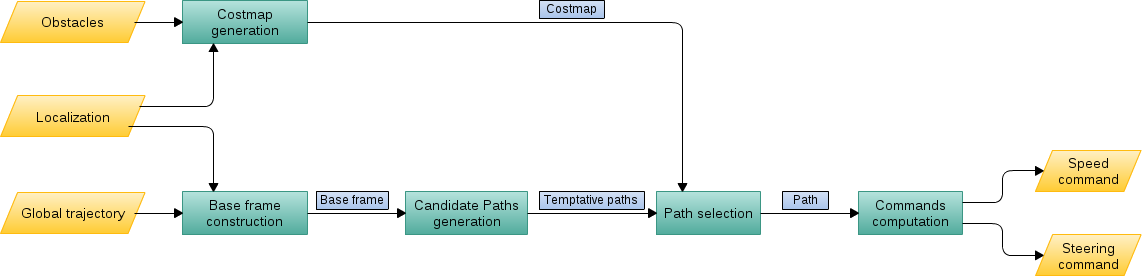
\includegraphics[width=\textwidth]{pipeline}
        \caption{Pipeline of the method described on this chapter.}\label{fig:cp07_pipeline}
\end{figure*}

\subsection{Generation of the costmap}\label{ch:chapter07_01_01}

The costmap maintains information about occupied/free areas in the map in the form of an occupancy grid. It uses sensor data and information from the static map to store and update information about obstacles in the world. In the tests shown in this chapter, information is obtained through the \acp{LIDAR}. Some tests including the information obtained from the methods described in previous sections will be shown at section \ref{ch:chapter08_07}. Each sensor is used to mark obstacles in the map, or clear them if they are no longer available (That is, if we find an obstacle that is clearly behind a previously detected obstacle, or the laser do not detect anything in this direction inside a given range, we assume that the obstacle disappeared).

Each cell in the map can have $255$ different cost values:
\begin{itemize}
 \item A value of $255$ means that we do not have information about an specific cell in the map.
 \item $254$ means that a sensor has marked this specific cell as occupied. This is considered as a lethal cell, so the vehicle should never enter there.
 \item The rest of cells are considered as free, but with different cost levels depending on an inflation method relative to the size of the vehicle and its distance to the obstacle.
\end{itemize}

Cost values out from occupied cells decrease with distance using the following expression:

\begin{equation}\label{eq:cp07_costmap_inflation}
 \mathcal{C}(i, j) = \exp (-1.0 \cdot \alpha \cdot ( \|c_{ij}-\vec{o}\| - \rho_{inscribed})) \cdot 253
\end{equation}

In this expression, which is the same we used in section \ref{ch:chapter06_01_01_01} of chapter \ref{ch:chapter06}, $\alpha$ is a scaling factor that allows increasing or decreasing the decay rate of the cost of the obstacle. $\|c_{ij}-\vec{o}\|$ is the distance between the cell $c_{ij} \in \mathcal{C}$ (where $\mathcal{C}$ is the set of cells in the costmap) and the obstacle. Finally, $\rho_{inscribed}$ is the inscribed radius, which is the inner circle of the limits of the car. This radius is depicted in the figure \ref{fig:cp07_costmap_concepts}.

\begin{figure}[h!]
\centering
\begin{tabular}{c}
  \begin{subfigure}[b]{\textwidth}
    \centering
    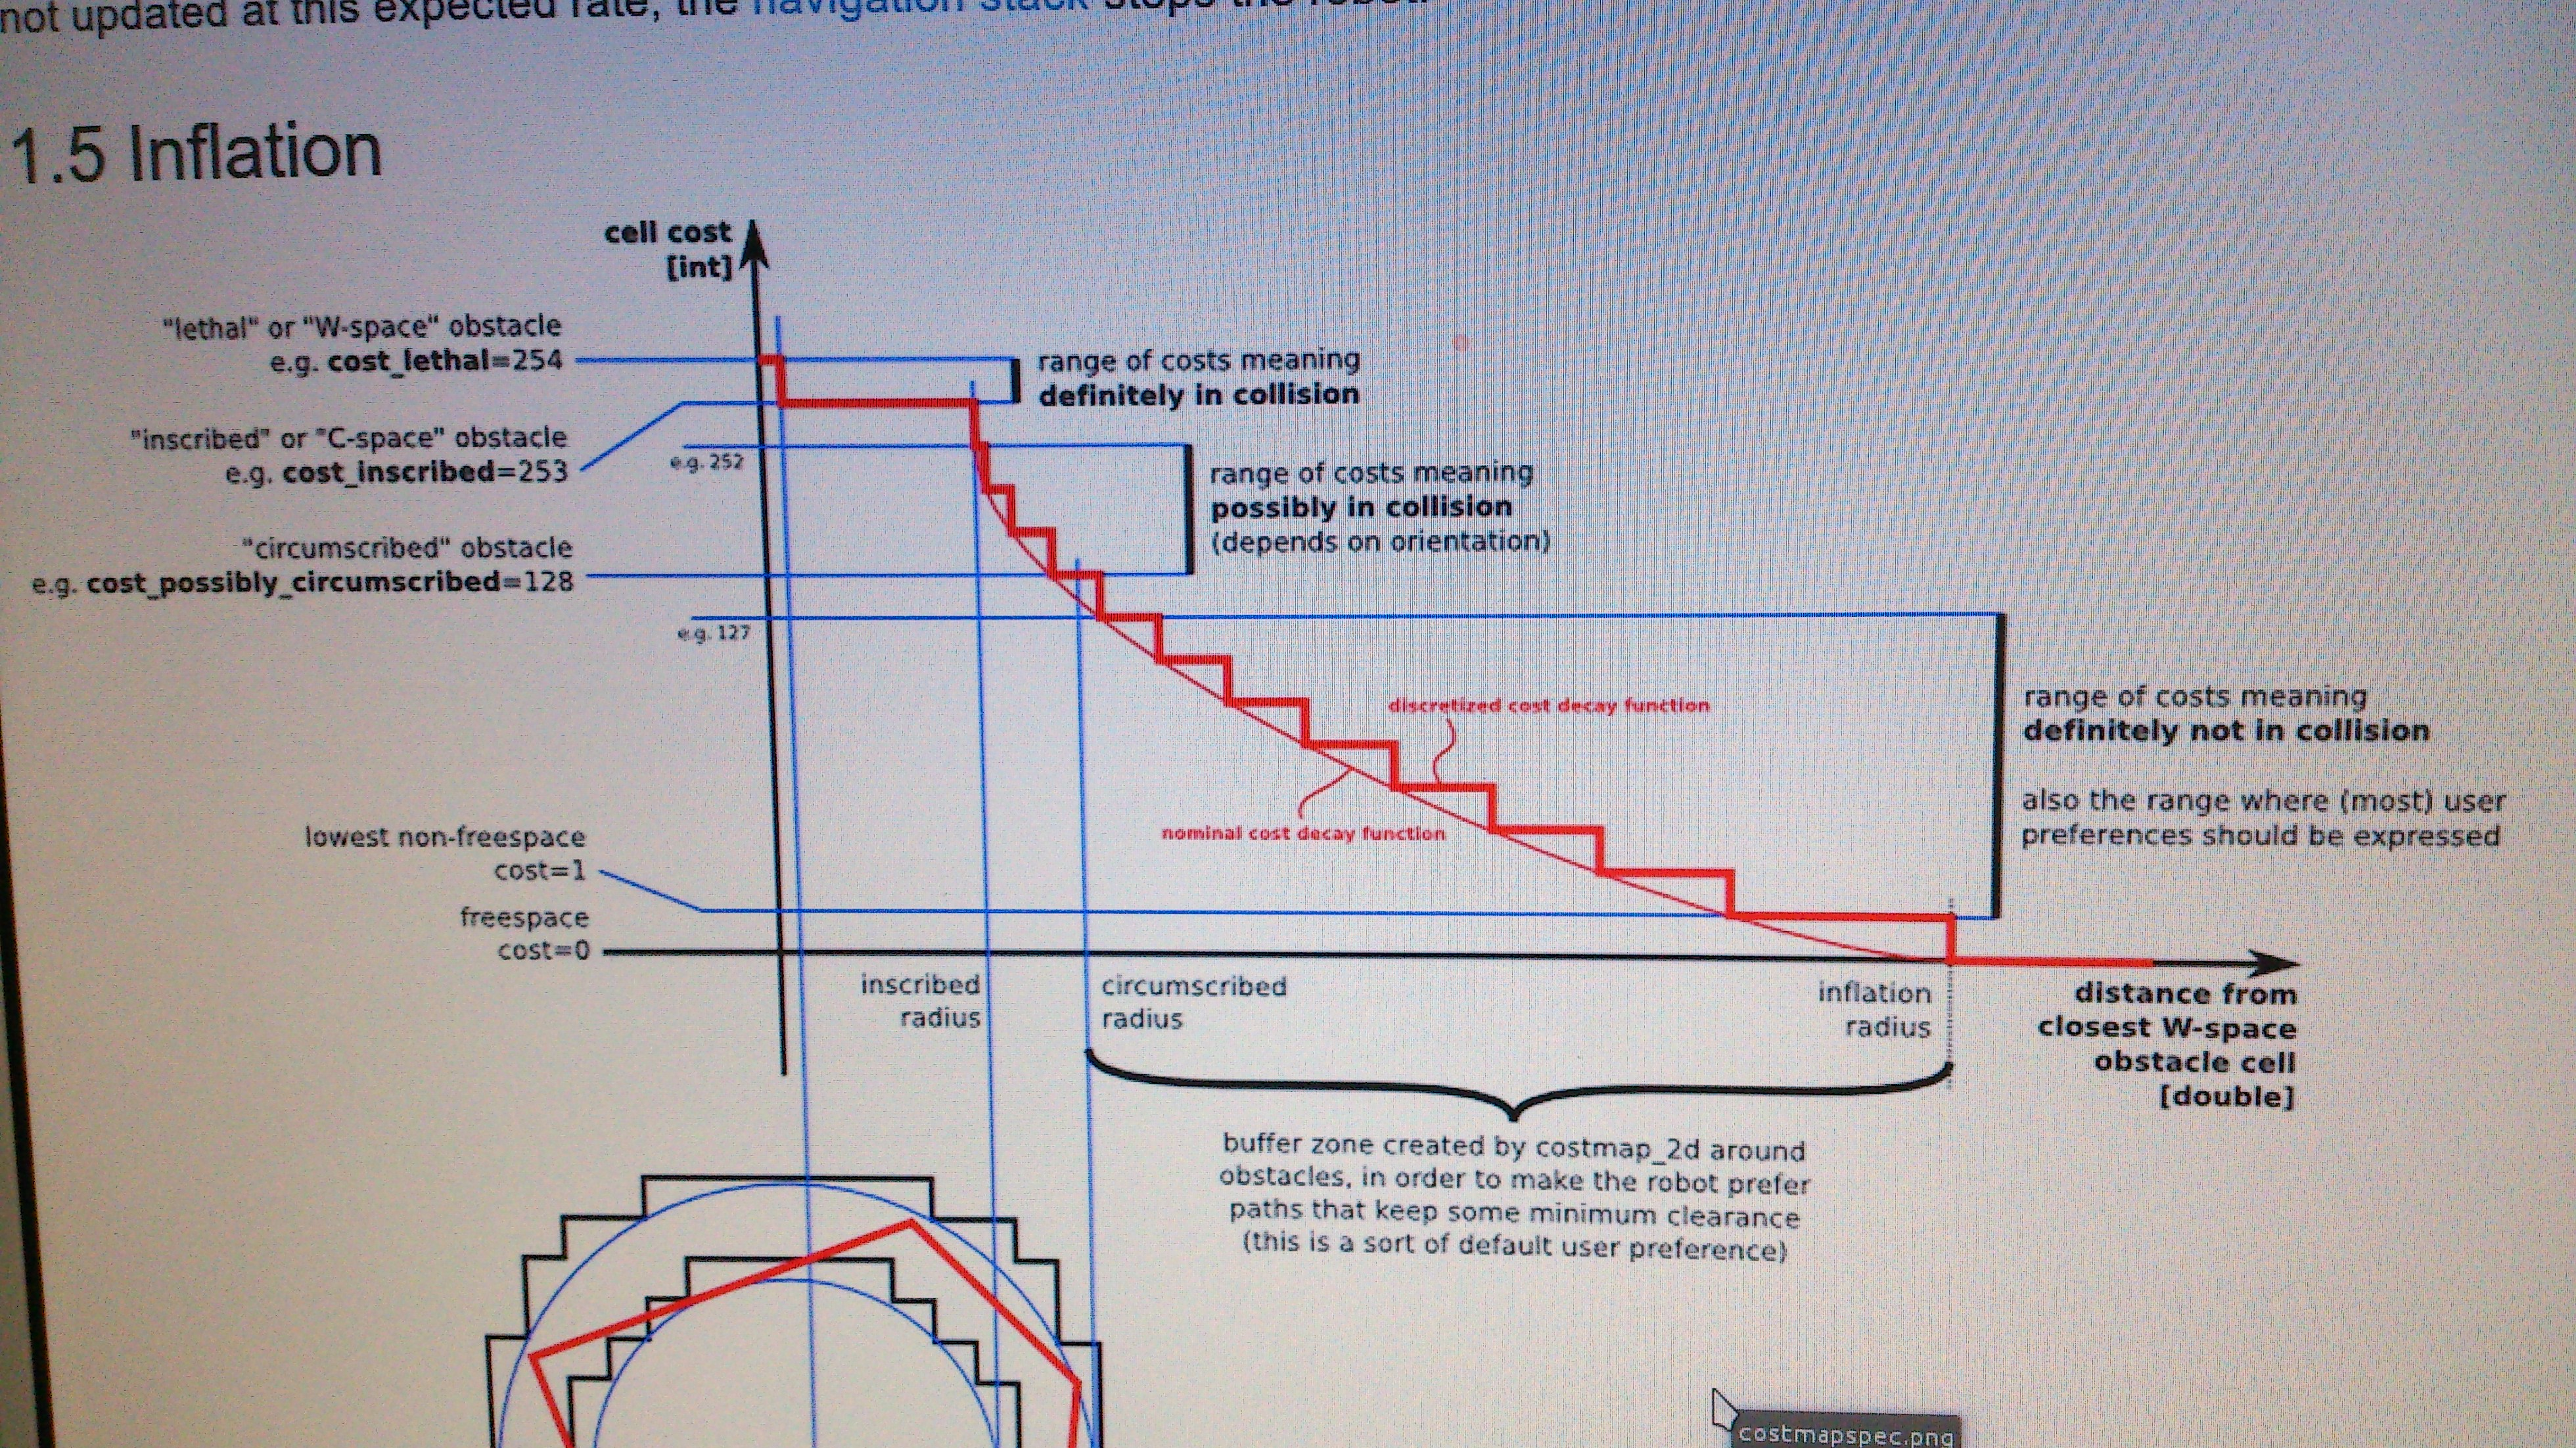
\includegraphics[width=\textwidth]{cost_levels}
    \caption{Cost levels.}
    \label{fig:cp07_cost_levels}
  \end{subfigure}\\ 
  \begin{subfigure}[b]{\textwidth}
    \centering
    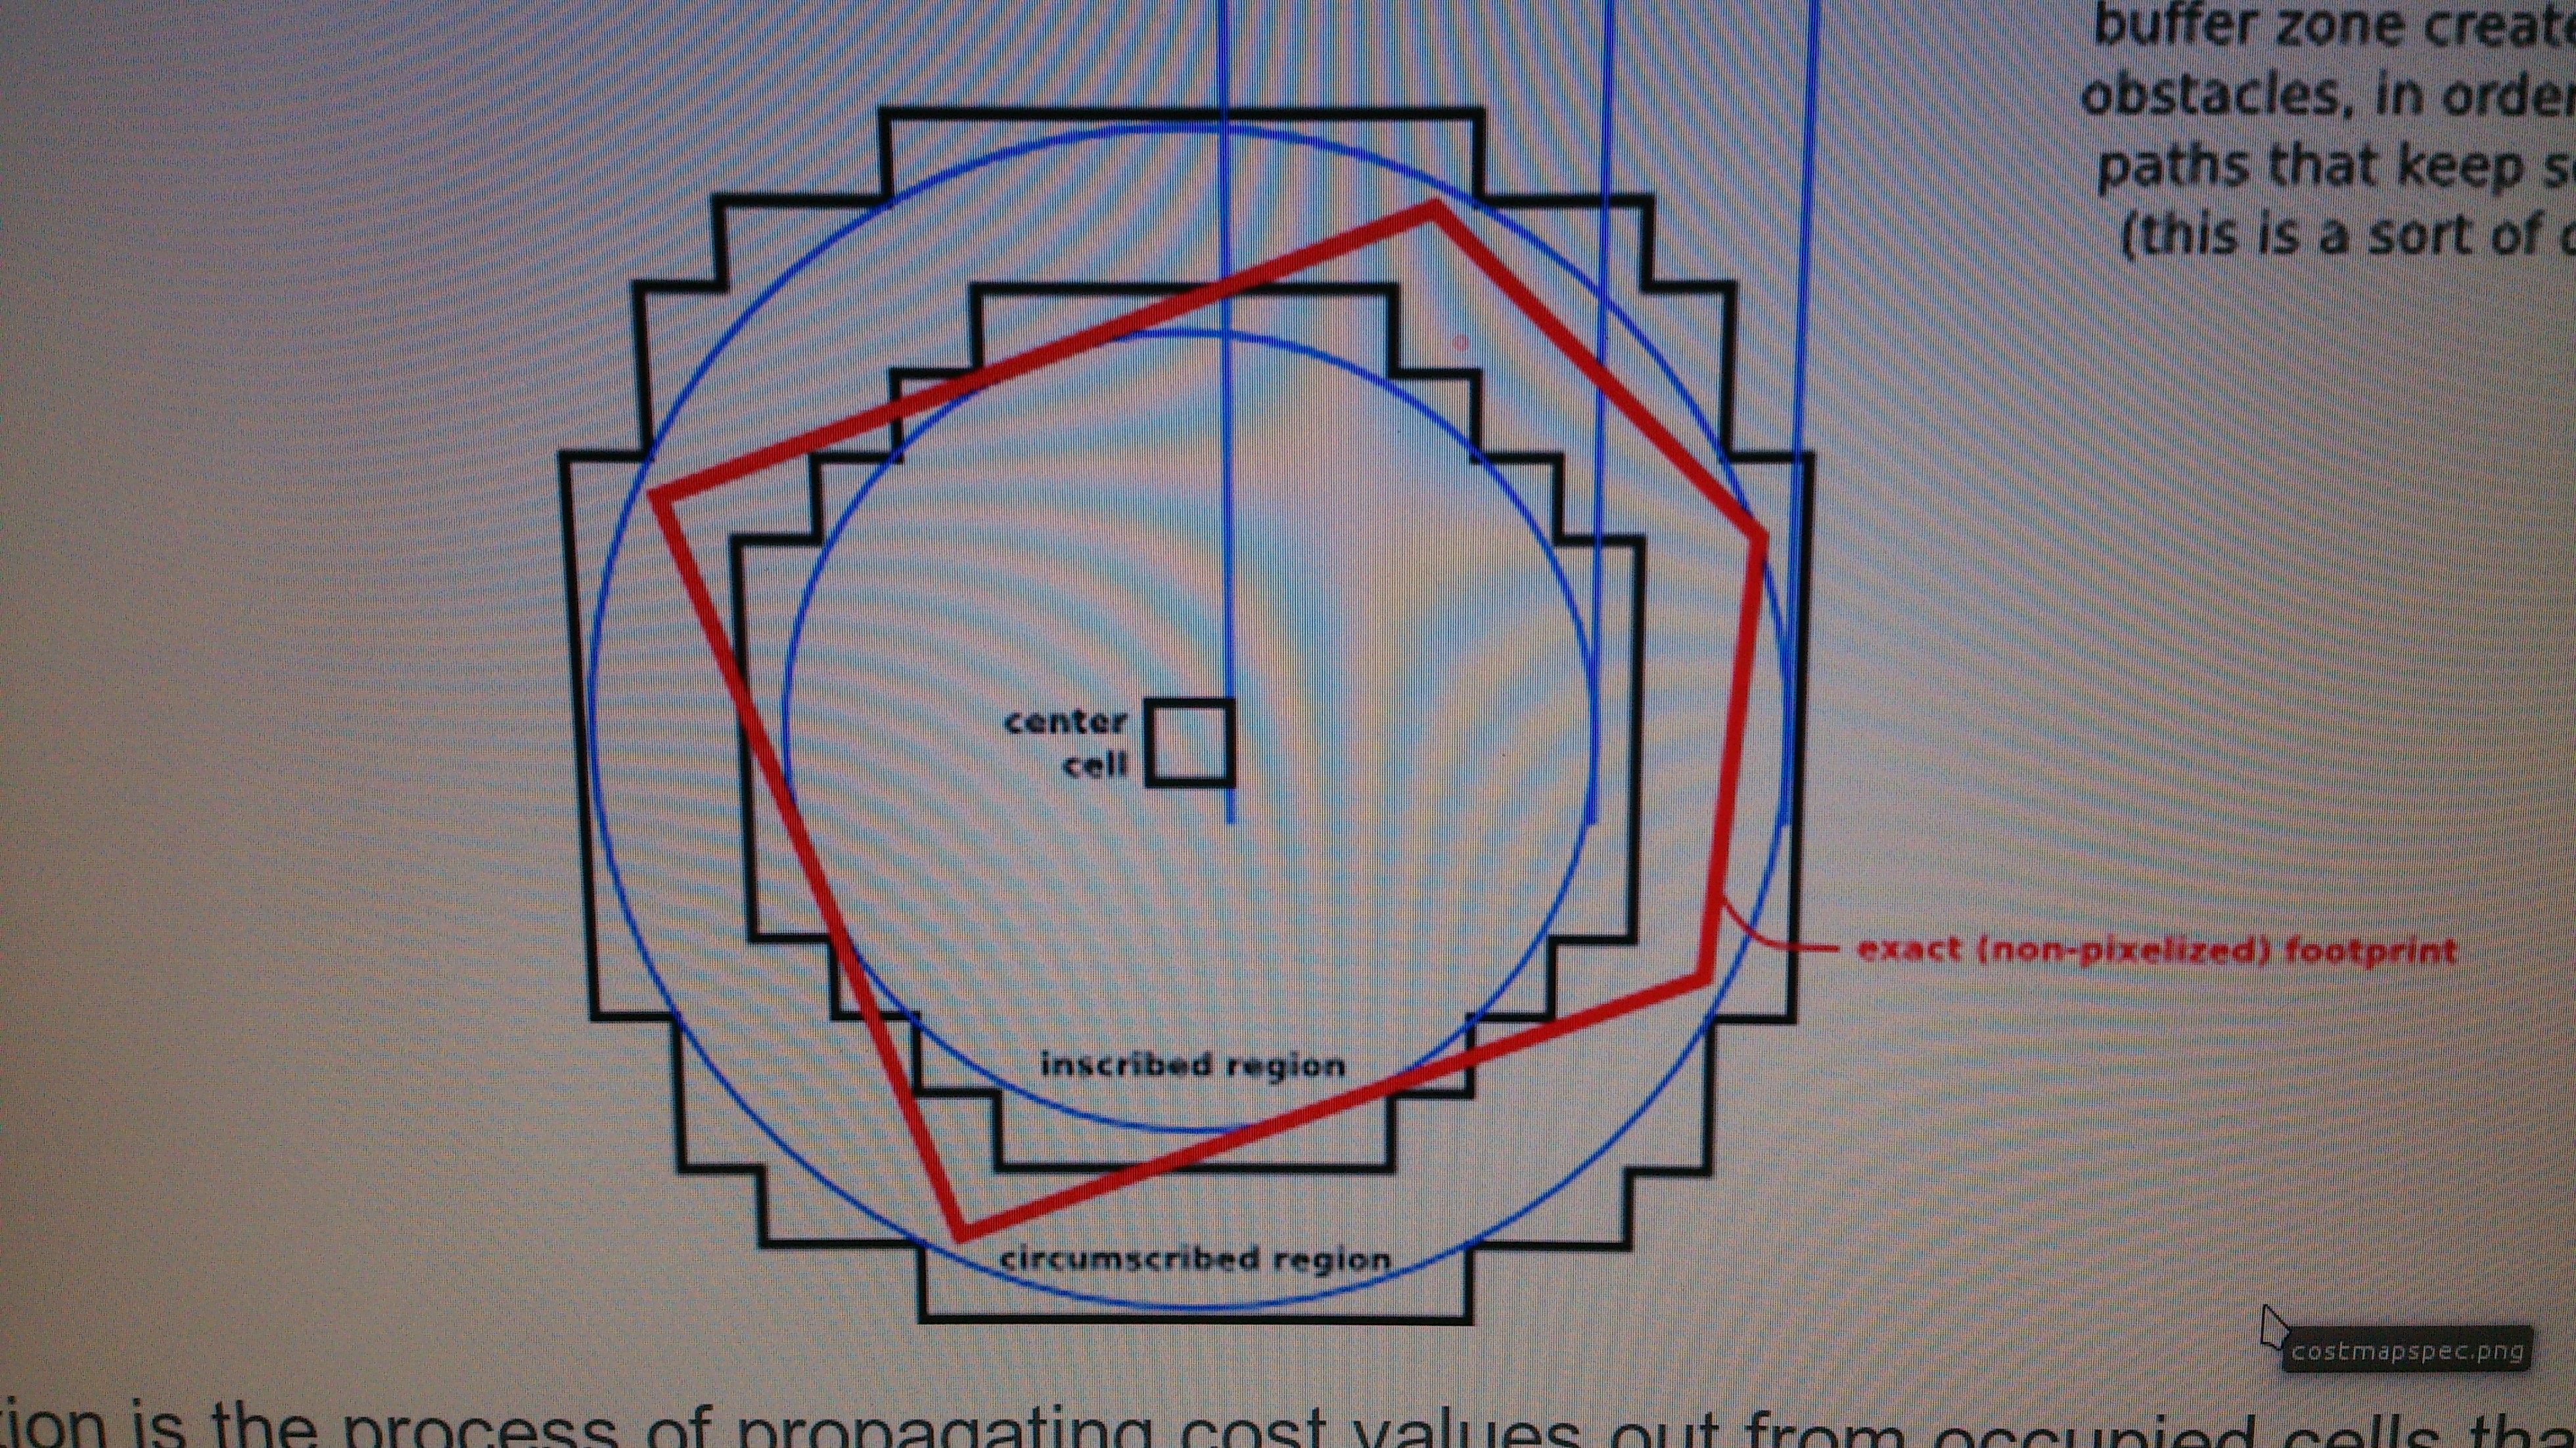
\includegraphics[width=\textwidth]{inscribed_circumscribed}
    \caption{$\rho_{inscribed}$ and $\rho_{circumscribed}$.}
    \label{fig:cp07_inscribed_circumscribed}
  \end{subfigure}
\end{tabular}
\caption{Costmap computation concepts.}\label{fig:cp07_costmap_concepts}
\end{figure}

Despite all of them are free cells, we define four different distance thresholds in order to set different danger levels in the map, depicted in figure \ref{fig:cp07_costmap_concepts}:

\begin{itemize}
 \item $\tau_{lethal}$: There is a obstacle in this cell, marked by the sensor. Corresponds to the cost level $254$. The vehicle is in collision.
 \item $\tau_{inscribed}$: The cell distance to the nearest obstacle is below the value $\rho_{inscribed}$. If the center of the vehicle is in this cell, it is also in collision, so the areas below this distance threshold should be avoided. The cost level is always $253$.
 \item $\tau_{circumscribed}$: If the vehicle center is on this cell, it is very likely that the car is in collision with an obstacle, depending on its orientation. A cell with a distance to an obstacle below this threshold should be avoided, but there still are chances of being in one of them without colliding an obstacle. 
 \item The rest of cells are assumed to be safe (except from those with \emph{unknown} cost, for which we do not know if they are occupied or not, so we think on them as if they were lethal).
\end{itemize}

In our approach, we just consider those paths passing through cells with a cost below $\tau_{circumscribed}$, which is obtained obtained using the equation \ref{eq:cp07_costmap_inflation} and other cost factors that will be explained later. Paths passing trough the cells over this threshold will be truncated at the last safe point.

For optimization reasons, we do not compute the costmap for the whole map at each iteration. Instead, we just compute the cells in a $40 \times 40\,m$ area centered into the current car position. 

In the development of this method, we used the \ROS plugin \program{costmap\_2d}\footnote{\url{http://wiki.ros.org/costmap\_2d}}, which implements the functionalities described in this section. \comment{¿Quitar?}

\subsection{Base frame construction}\label{ch:chapter07_01_02}

Before the construction of the base frame, we must find the point we want to use as origin of coordinates. At each iteration,  we prune the global plan up to its nearest point to the car location. The origin of the base frame will be the first point in the pruned global plan. If the pruned plan is valid and its size is different from zero, we start the base frame construction stage.

In this stage, we will define the base frame of the curvilinear coordinate system, so the algorithm will be able to compute the trajectories in this space as if the global plan were a rectilinear trajectory. The geometric relationship between the path in euclidean and curvilinear coordinates is shown at figure \ref{fig:cp07_euclidean_frenet_conversion}.

\begin{figure}[h!]
\centering
\begin{tabular}{cc}
  \begin{subfigure}[b]{0.45\textwidth}
      \centering
      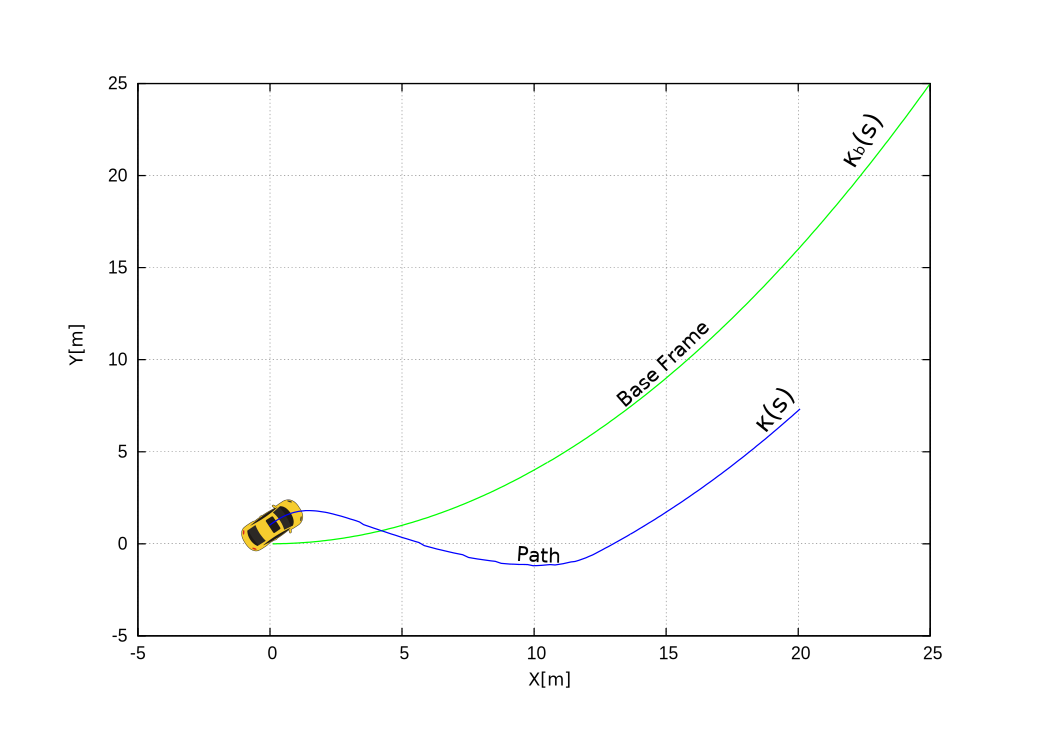
\includegraphics[width=\textwidth, trim=50 30 80 60,clip]{justOneCartesian45}
      \caption{Euclidean space.}
      \label{fig:cp07_justOneCartesian45}
  \end{subfigure} &
  \begin{subfigure}[b]{0.45\textwidth}
    \centering
    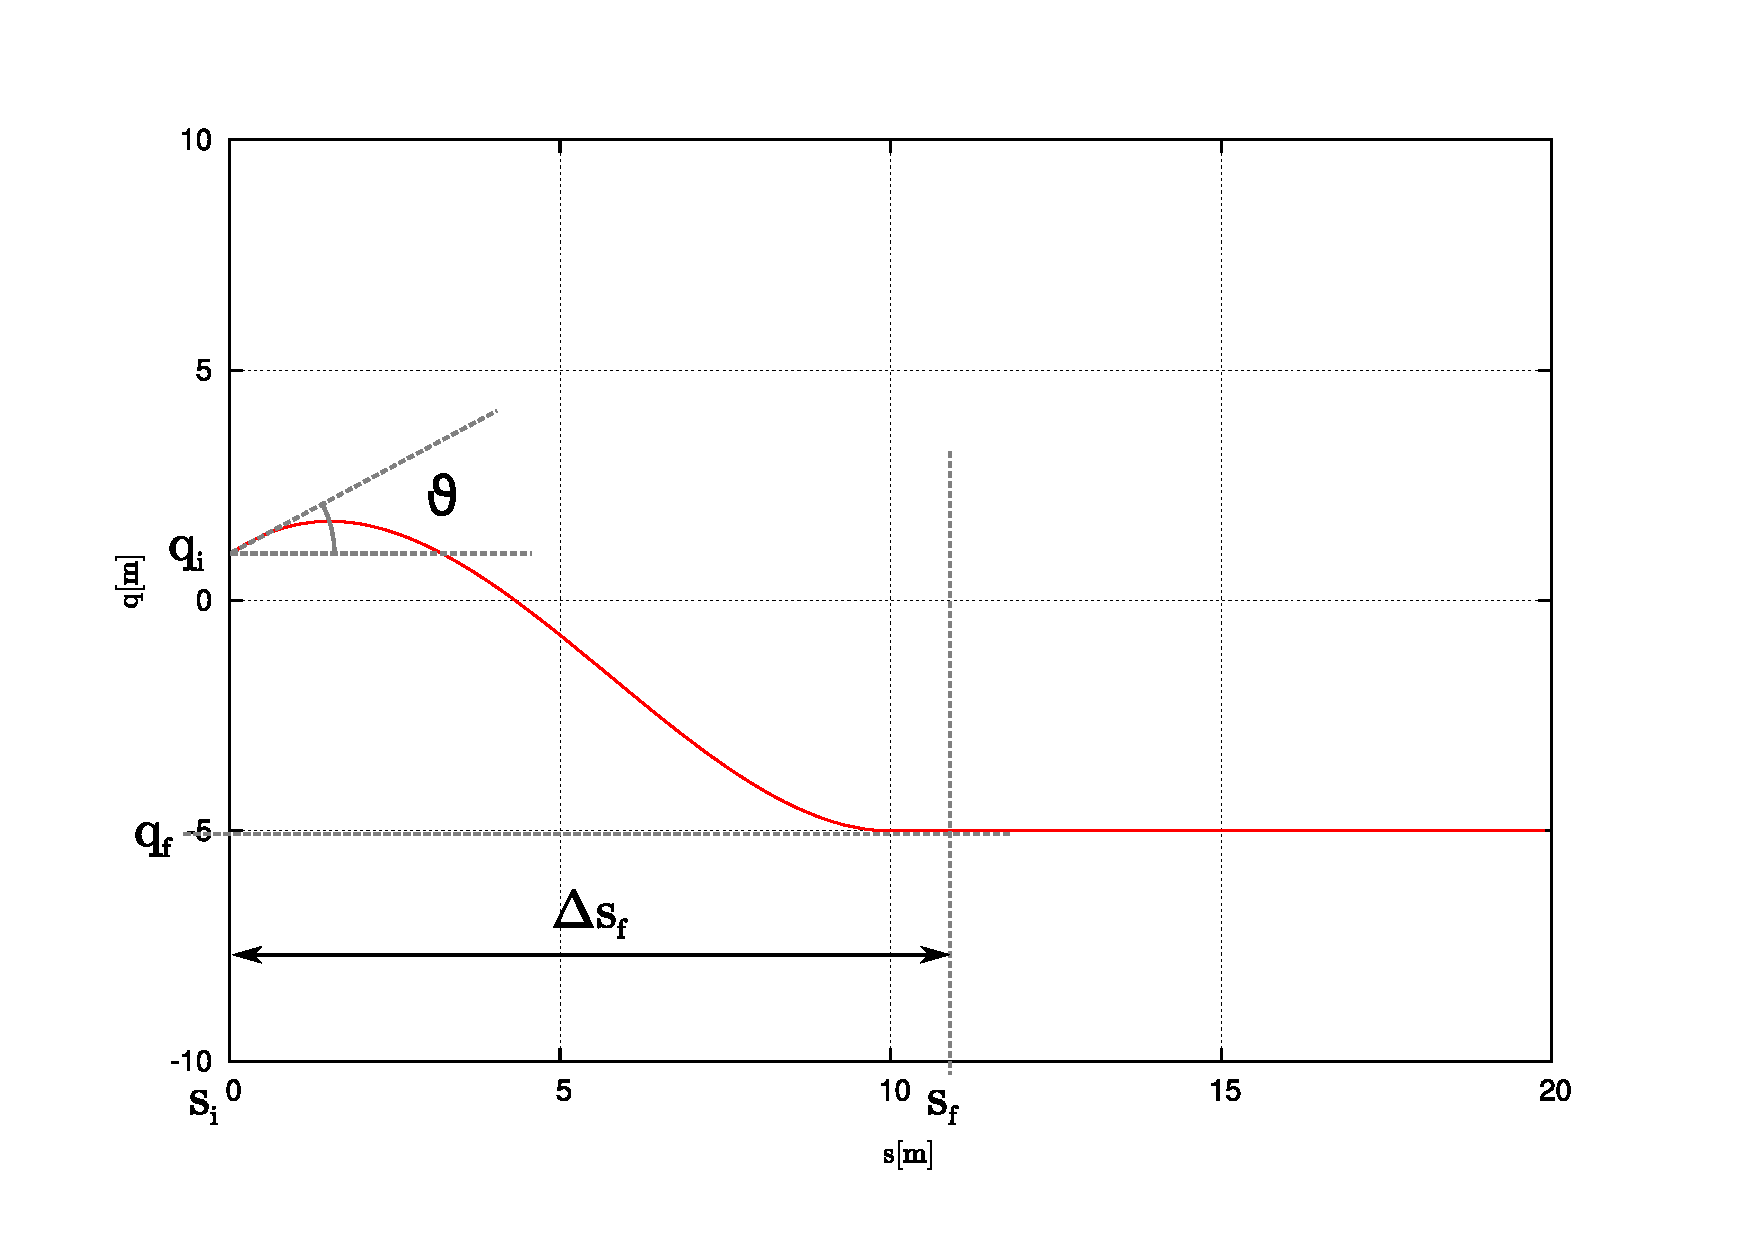
\includegraphics[width=\textwidth, trim=50 30 80 60,clip]{justOneFrenet45}
    \caption{Curvilinear space.}
    \label{fig:cp07_justOneFrenet45}
  \end{subfigure}%   
\end{tabular}
\caption{Conversion of a trajectory between the Cartesian and Frenét spaces.}\label{fig:cp07_euclidean_frenet_conversion}
\end{figure}

There, the longitude of the arc of the base frame ($s$, on the right image) is the distance along the global plan, which is represented as a green line. This distance is represented by the horizontal axis of the curvilinear system. The vertical axis, $q$, represents the perpendicular lateral distance respect to the path. Left side is represented by positive values and the right by the negatives.

For the computation of the transformation between the euclidean coordinate system and the curvilinear, we need to compute $\kappa$, that represents the path curvature. This value is computed as follows \citep{chu2012local, werling2010optimal, barfoot2004motion}:

\begin{equation}\label{eq:cp07_path_curvature}
 \kappa = {S \over Q} \cdot \left ( \kappa_b \cdot { 
 {(1 - q \cdot \kappa_b) \cdot (\partial^2q / \partial s^2) +
 \kappa_b \cdot (\partial q / \partial s )^2
 } 
 \over {Q^2} } \right )
\end{equation}

,where 

\begin{equation}\label{eq:cp07_path_curvature_s_and_q}
\begin{cases}
S=sign(1 - q \cdot \kappa_b)\\
Q=\sqrt{\left ( { {\partial q} \over {\partial s}} \right ) ^2+ (1 - q \cdot \kappa_b)^2}
\end{cases}
\end{equation}

A generated path will be rejected in the following cases:

\begin{itemize}
 \item The lateral offset $q$ is similar to the curvature radius of the base frame $1 / \kappa_b$. In this case, the path passes through the center of curvature of the base frame.
 \item $q > {1 \over \kappa_b}$. In this case, the generated path curvature and sense is opposed to that of the base frame. The path violates the non-holonomic condition of the movement of the vehicle, so it is discarded.
\end{itemize}

Also, the maximal curvature a path can have in order to be feasible by the vehicle is limited by the maximal steering angle. If this restriction is violated, the corresponding path is rejected. Curvature is directly related to the movement of the vehicle, which can be described through several models. A simplified version  \citep{chu2012local, barfoot2004motion}, which ignores the related physical effects (like inertia or mass), is:

\begin{equation}\label{eq:cp07_simplified_motion_model}
\begin{cases}
\dot{x} = |\vec{v}| \cdot cos(\theta) \\
\dot{y} = |\vec{v}| \cdot sin(\theta) \\
\dot{\theta} = |\vec{v}| \cdot \kappa
\end{cases}
\end{equation}

As these physical effects do not affect to the geometric shape of the path, we can ignore them in the path generation step. In equation \ref{eq:cp07_simplified_motion_model}, $[\dot{x} ~ \dot{y} ~ \dot{\theta} ]^T$ are the estimated position and orientation of the vehicle and $|\vec{v}|$ is speed magnitude. Considering this simplified model, we assume that the vehicle just have two degrees of freedom, represented by the speed $\vec{v}$ and $\kappa$. As we are just interested into the geometric generation of the path, it is possible to remove the speed of the vehicle $\vec{v}$ from the model. This is done by expressing the movement of the vehicle in terms of the traveled distance. So the following relation is established \citep{chu2012local}:

\begin{equation}\label{eq:cp07_speed_to_distance}
|\vec{v}| = S \cdot Q \cdot { {\partial s} \over {\partial t}}
\end{equation}

If the speed of the vehicle is substituted into the model described in equation \ref{eq:cp07_simplified_motion_model}, the differential equation of the movement can be represented in terms of the base frame's arc length:

\begin{equation}\label{eq:cp07_motion_model_in_distance_terms}
\begin{cases}
{{\partial x} \over {\partial s}} = Q \cdot cos(\theta) \\
{{\partial y} \over {\partial s}} = Q \cdot sin(\theta) \\
{{\partial \theta} \over {\partial s}} = Q \cdot \kappa
\end{cases}
\end{equation}

\subsection{Candidate paths generation}\label{ch:chapter07_01_03}

As seen, path generation is performed in the curvilinear space, without considering the obstacles in the environment. These will be taken into account later, once the tentative trajectories are transformed to the euclidean space.

\subsubsection{Maneuvering paths generation}\label{ch:chapter07_01_03_01}

The curvature of the generated paths is defined by the lateral offset $q$ respect to the base frame. First and second order derivatives of $q$ are needed if we want to compute $\kappa$ (see equations \ref{eq:cp07_path_curvature} and \ref{eq:cp07_path_curvature_s_and_q}), so we need a function dependent on the lateral offset if we want to compute a smooth lateral change.

$q$ can be defined by a sequence of a cubic polynomial and a set of constants \citep{chu2012local}:

\begin{equation}\label{eq:cp07_function_q}
\begin{align*}
q(s) &=
  \begin{cases}
   a \cdot \Delta s^3 + b \cdot \Delta s^2 + c \cdot \Delta s + q_i & \text{if } s_i \le s < s_f \\
   q_f        & \text{if } s_f \le s
  \end{cases}\\
{{\partial q} \over {\partial s}}(s) &=
  \begin{cases}
   3 \cdot a \cdot \Delta s^2 + 2 \cdot b \cdot \Delta s + c & ~~~~~~~\text{if } s_i \le s < s_f \\
   0        & ~~~~~~~\text{if } s_f \le s
  \end{cases}\\
{{\partial^2 q} \over {\partial s^2}}(s) &=
  \begin{cases}
   6 \cdot a \cdot \Delta s + 2 \cdot b & ~~~~~~~~~~~~~~~~~~~~~~~\text{if } s_i \le s < s_f \\
   0        & ~~~~~~~~~~~~~~~~~~~~~~~\text{if } s_f \le s
  \end{cases}
\end{align*}
\end{equation}

, where $\Delta s = s - s_i$.

In figure \ref{fig:cp07_justOneFrenet45}, the components involved in this process are depicted.
\begin{itemize}
 \item The initial lenght $s_i$ is zero, due to the pruning process performed at the beginning of each iteration (section \ref{ch:chapter07_01_02}). Lateral offset $q_i$ is also known, which is the lateral offset respect to the global path's origin.
 \item Angle $\theta$ defines the difference between the vehicle heading angle and the tangent angle of the base frame at the current position.
 \item $s_f$ is a parameter that allows controlling the longitudinal distance needed to reach the offset $q_f$. This distance should be dependent from the speed. However, as the maximal speed of the prototype is not too hight, we can think on $\Delta s_f$ as the distance needed to go from $q_i$ to the biggest $q_f$ at the maximal speed.
 \item The different $q_f$ are computed separately for each path attending to the parameters defined by the user. $s_f$ is also a free parameter.
\end{itemize}

Parameters $s_i$, $q_i$, and $s_f$ are shared by all the candidate paths. By modifying the value of $q_f$ we get the different tentative trajectories, so the only difference between all them is the lateral offset we want to reach at the end of the paths. This lateral offset will give us flexibility in the the way in which we avoid the obstacles. To do that, we divide the width of the road into as many segments as paths are desired. $q_f$ will be the perpendicular distance between the base frame and the corresponding road width division. Using this technique, the desired number of paths is created. The set of paths should cover the whole road width, ensuring the vehicle is able to avoid the obstacles, if it is possible.

In our tests, we have considered a maximal width of 4\,m (a little bit above the width of the roads in our testing area), and an horizon of 10\,m in the direction of the global path. This horizon gives us a prediction of 2\,seconds at the maximal speed of the vehicle. We evaluate a total of 21 paths, with a distance between them ($\Delta q_f$) of 20\,cm.

\subsubsection{Candidate paths generation}\label{ch:chapter07_01_03_02}

Once we have computed the paths in the curvilinear coordinate system, we transform them so we can work in the euclidean space. In this new space, we will be able to evaluate their associated costs, as those related to the distance to obstacles, smoothness, etc. In figures \ref{fig:cp07_frenet0} and \ref{fig:cp07_frenet45}, we can see two examples of this process.

In figure \ref{fig:cp07_frenet0}, an example in which the vehicle is at a lateral distance of 1\,m respect to the base frame, and the orientation of the vehicle regarding to this base frame is 0 is shown. That is, $q_i = 1$, $s_i = 0$ and $\theta = 0$. In the left image, we see that the set of paths is symmetric, being the central path completely parallel to the axis $s$. These trajectories are then projected to the euclidean space, obtaining the paths represented in the right image. There, the green line represents the global path, and the blue lines are the projected candidate paths. As shown, they fit properly to the global path.

\begin{figure}[h!]
\centering
\begin{tabular}{cc}
  \begin{subfigure}[b]{0.45\textwidth}
    \centering
    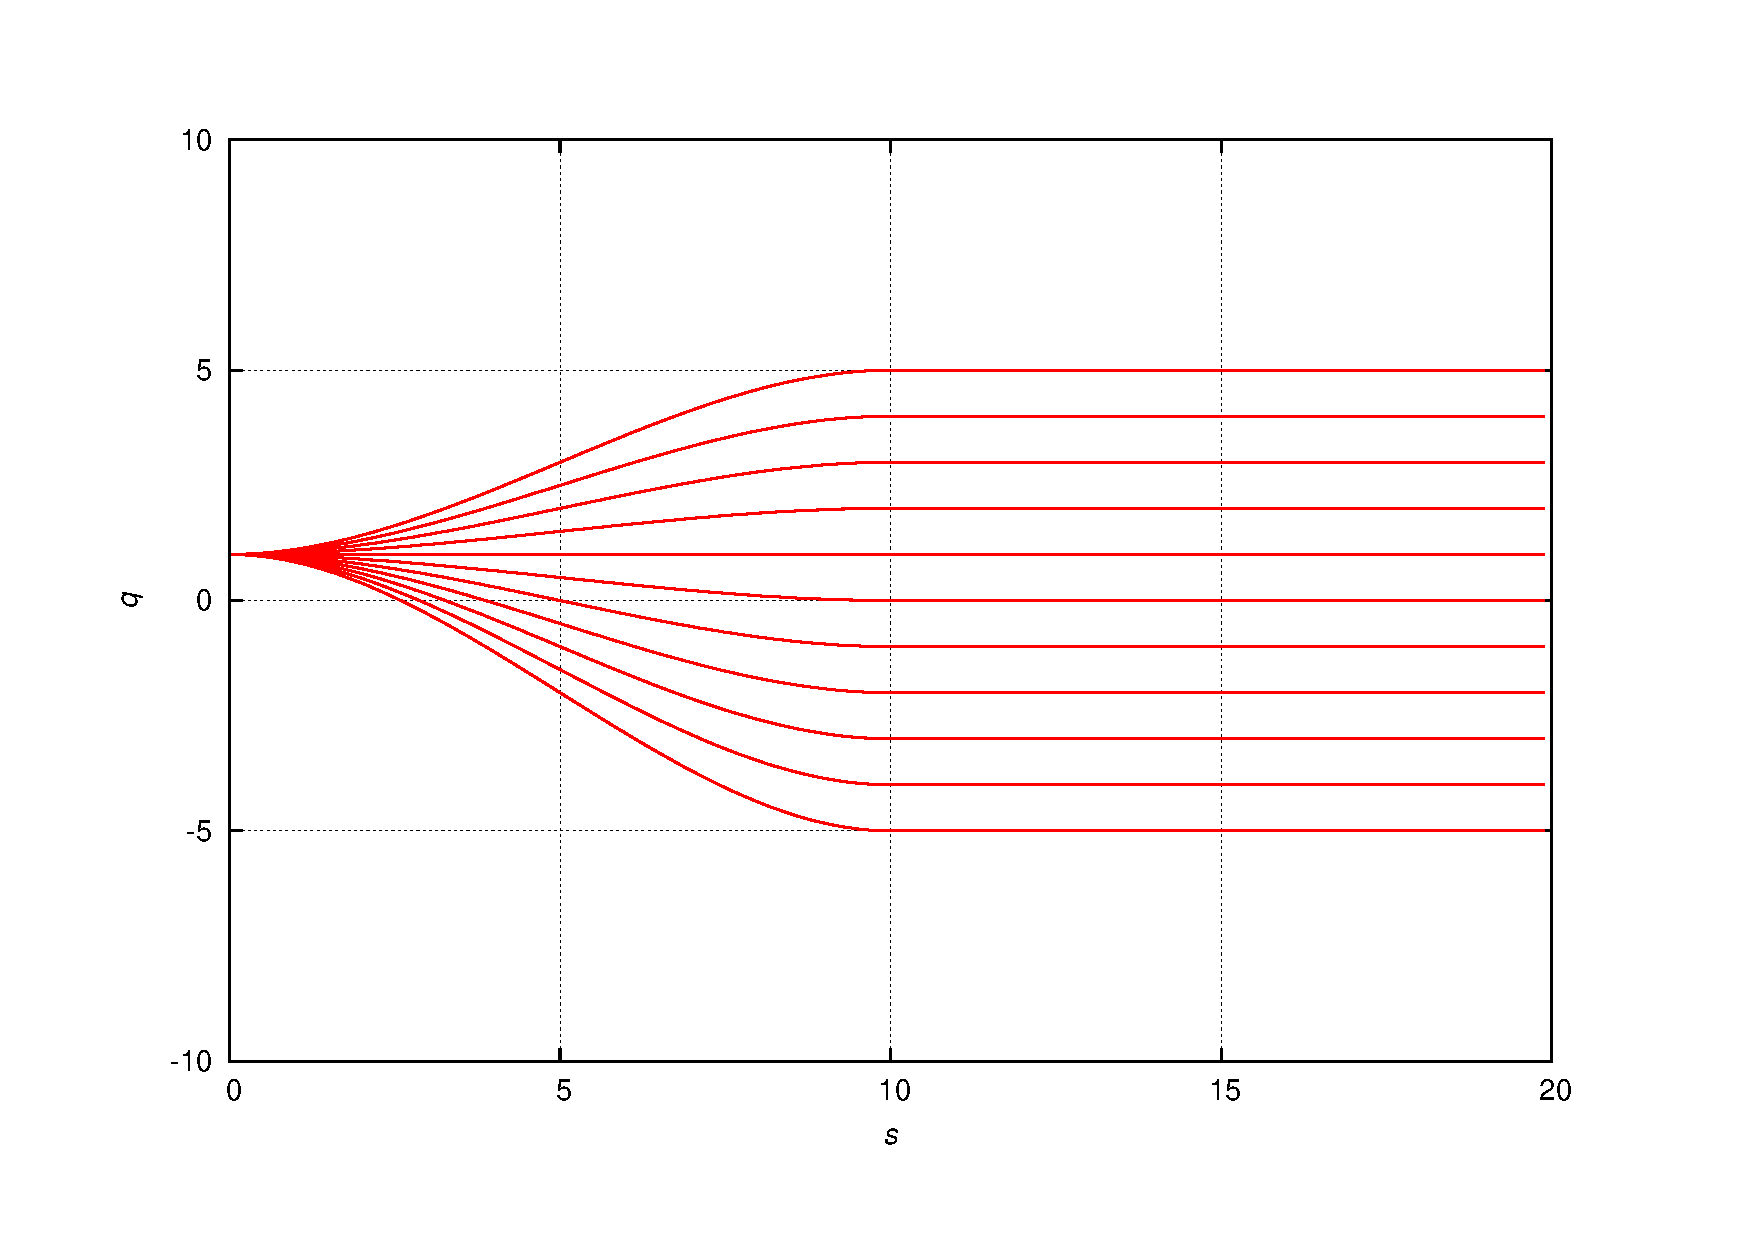
\includegraphics[width=\textwidth, trim=50 40 80 60,clip]{frenet0}
    \caption{Curvilinear space.}
    \label{fig:cp07_frenet0}
  \end{subfigure} &
  \begin{subfigure}[b]{0.45\textwidth}
    \centering
    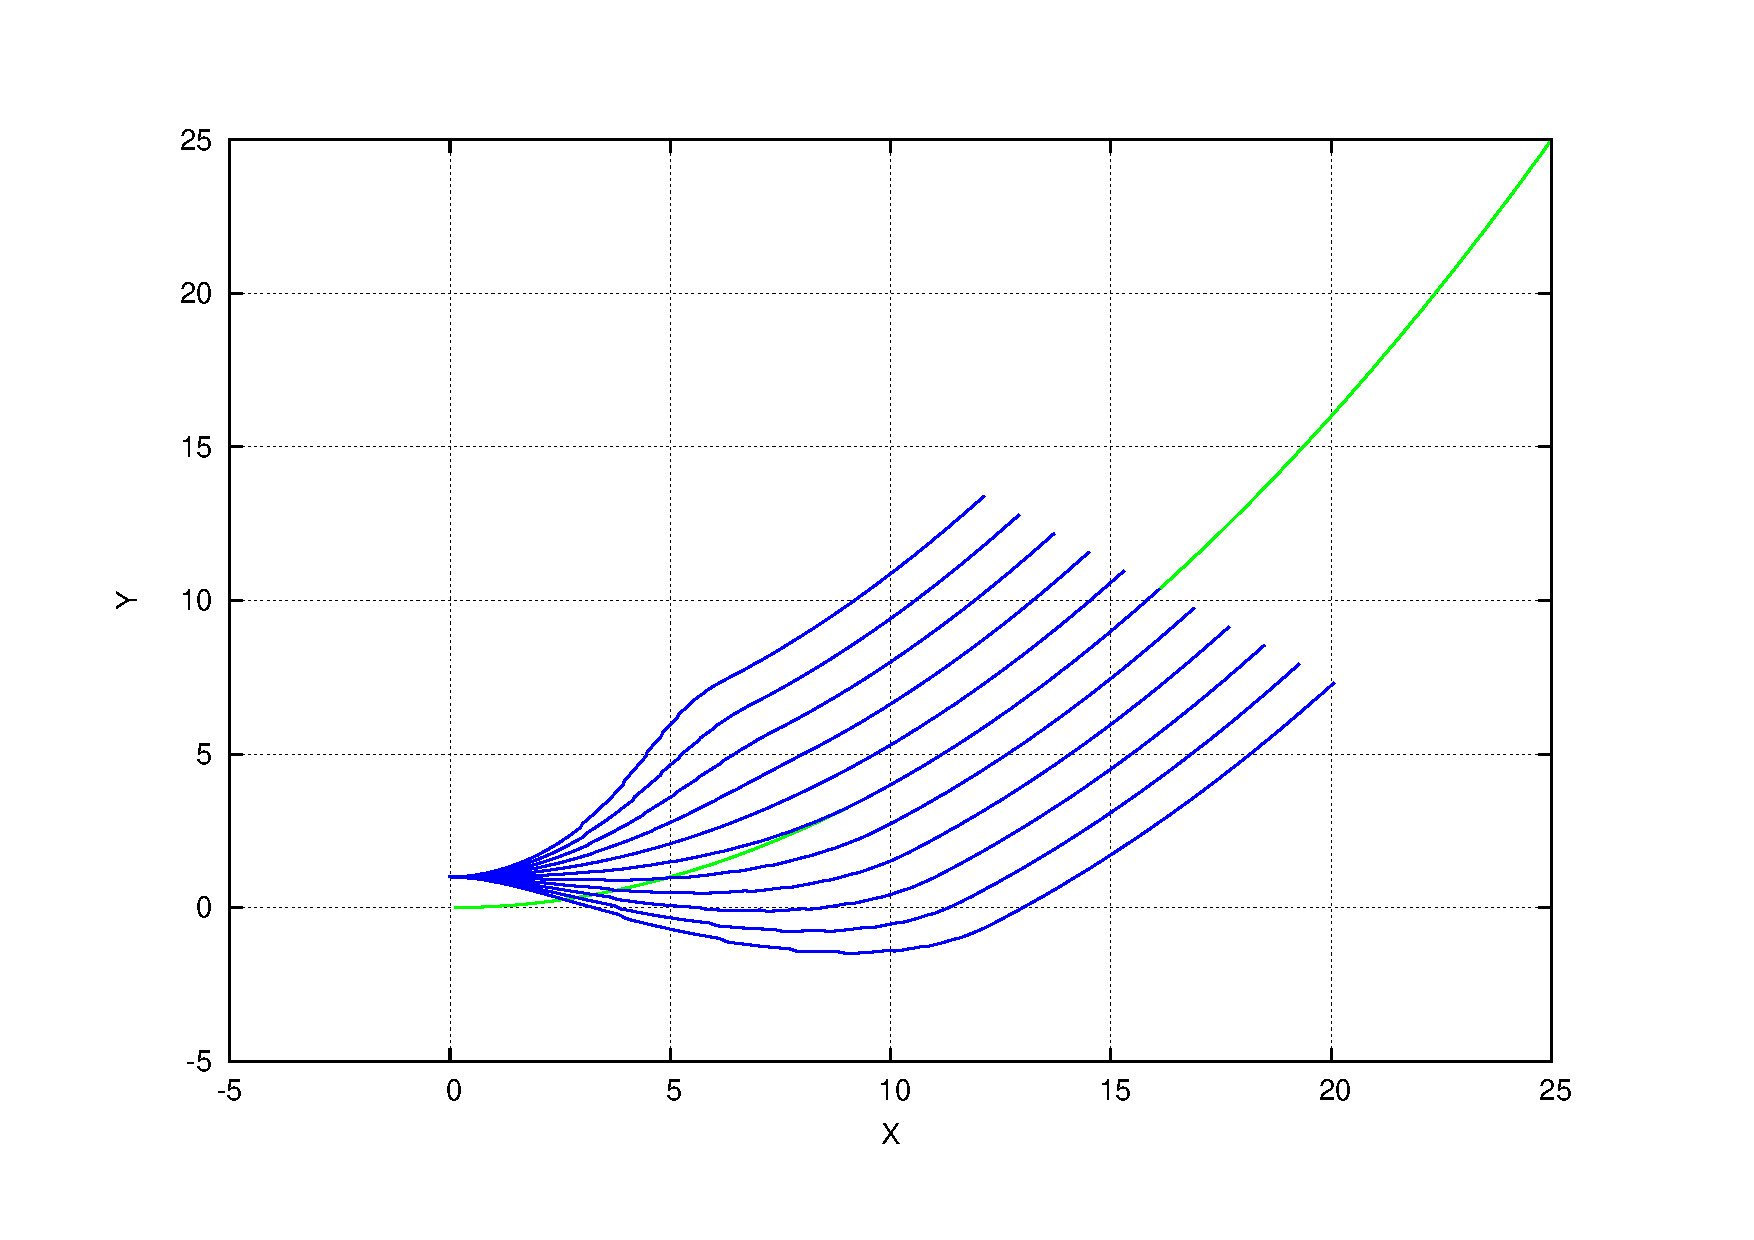
\includegraphics[width=\textwidth, trim=50 40 80 60,clip]{cartesian0}
    \caption{Euclidean space.}
    \label{fig:cp07_cartesian0}
  \end{subfigure}%
\end{tabular}
\caption{Example in which the vehicle is oriented parallel to the path.}\label{fig:cp07_frenet0}
\end{figure}

In figure \ref{fig:cp07_frenet45}, a similar example is shown. The only difference is that, this time, the vehicle is oriented $45^\circ$ away from the base frame orientation. This causes the paths in the curvilinear space to move away from the $s$ axis until they start converging. As shown, same effect occurs in the transformed euclidean paths: they move away from the global path but, after a few meters, they start approaching to it.

\begin{figure}[h!]
\centering
\begin{tabular}{cc}
  \begin{subfigure}[b]{0.45\textwidth}
    \centering
    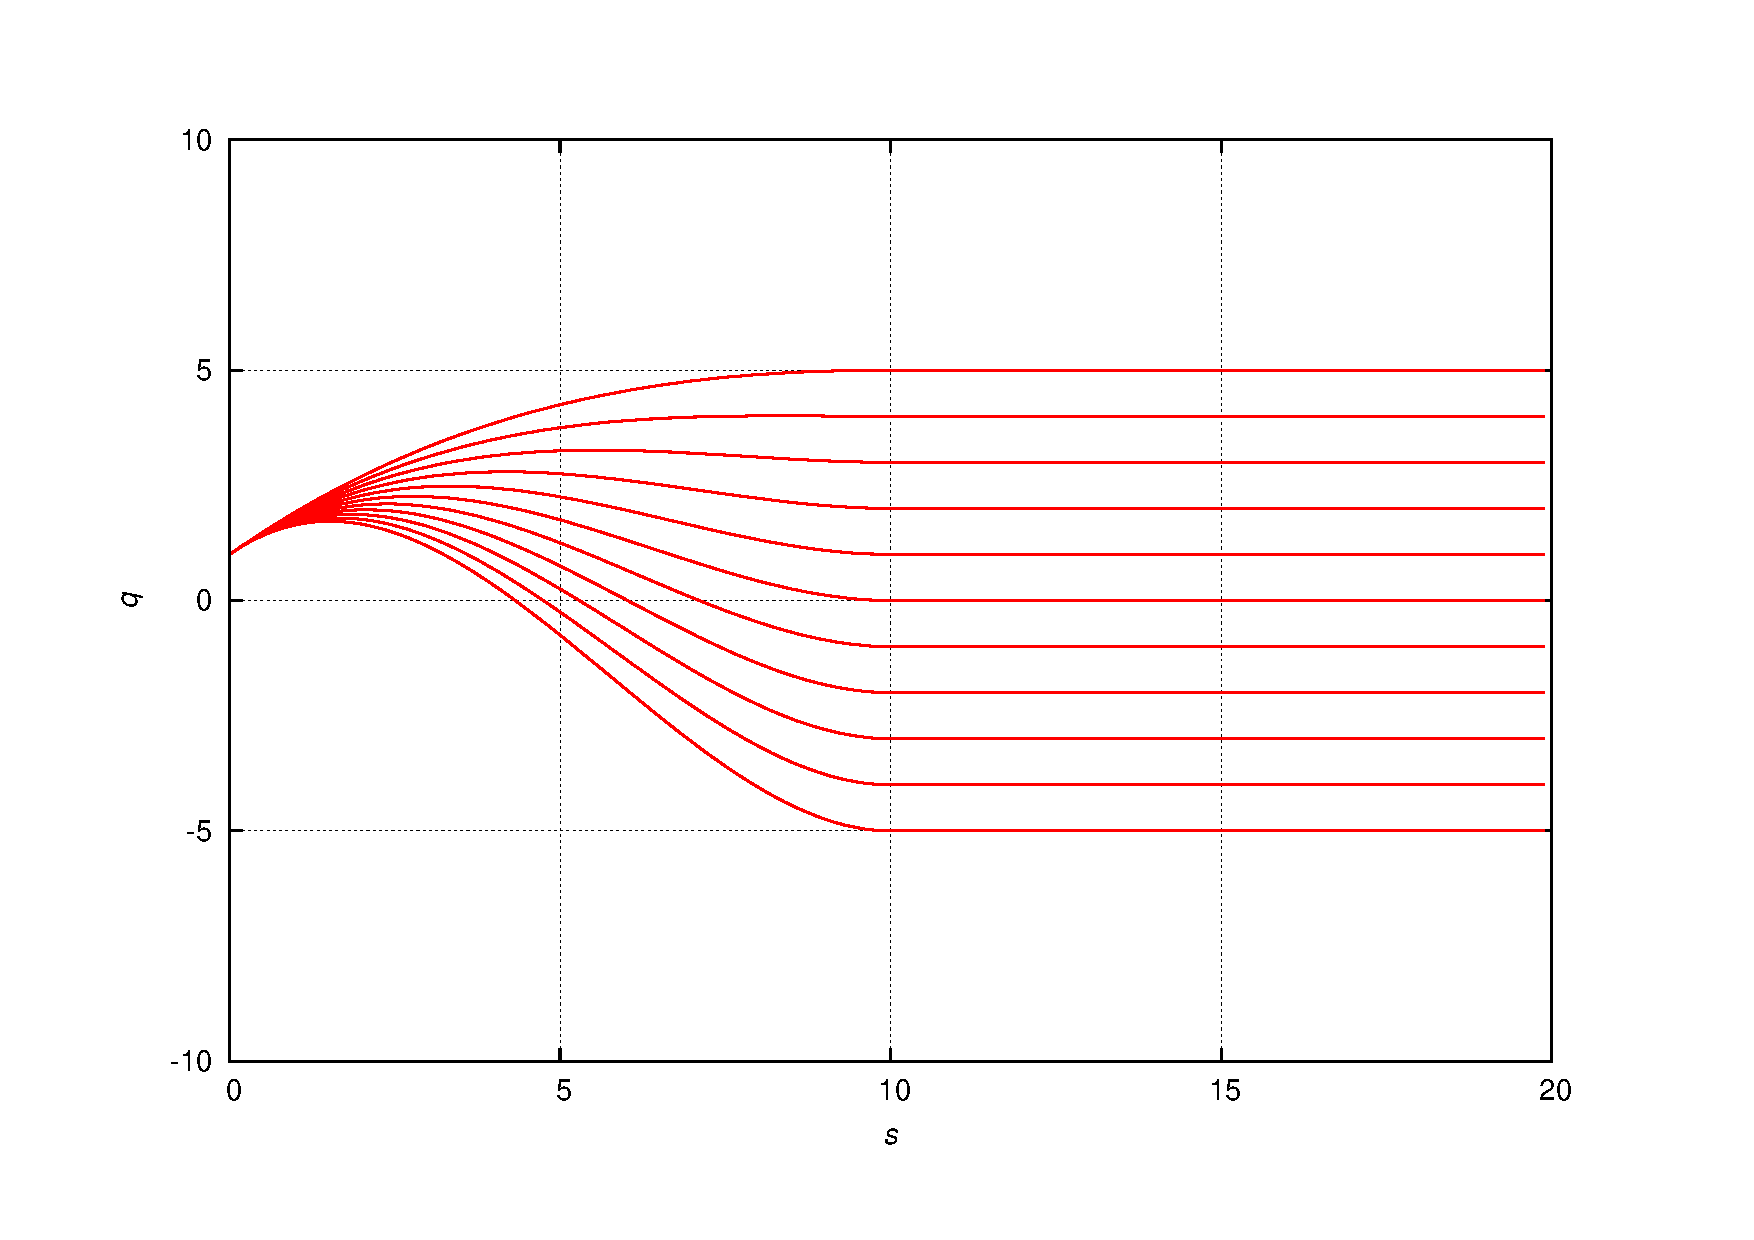
\includegraphics[width=\textwidth, trim=50 40 80 60,clip]{frenet45}
    \caption{Curvilinear space.}
    \label{fig:cp07_frenet45}
  \end{subfigure} &
  \begin{subfigure}[b]{0.45\textwidth}
    \centering
    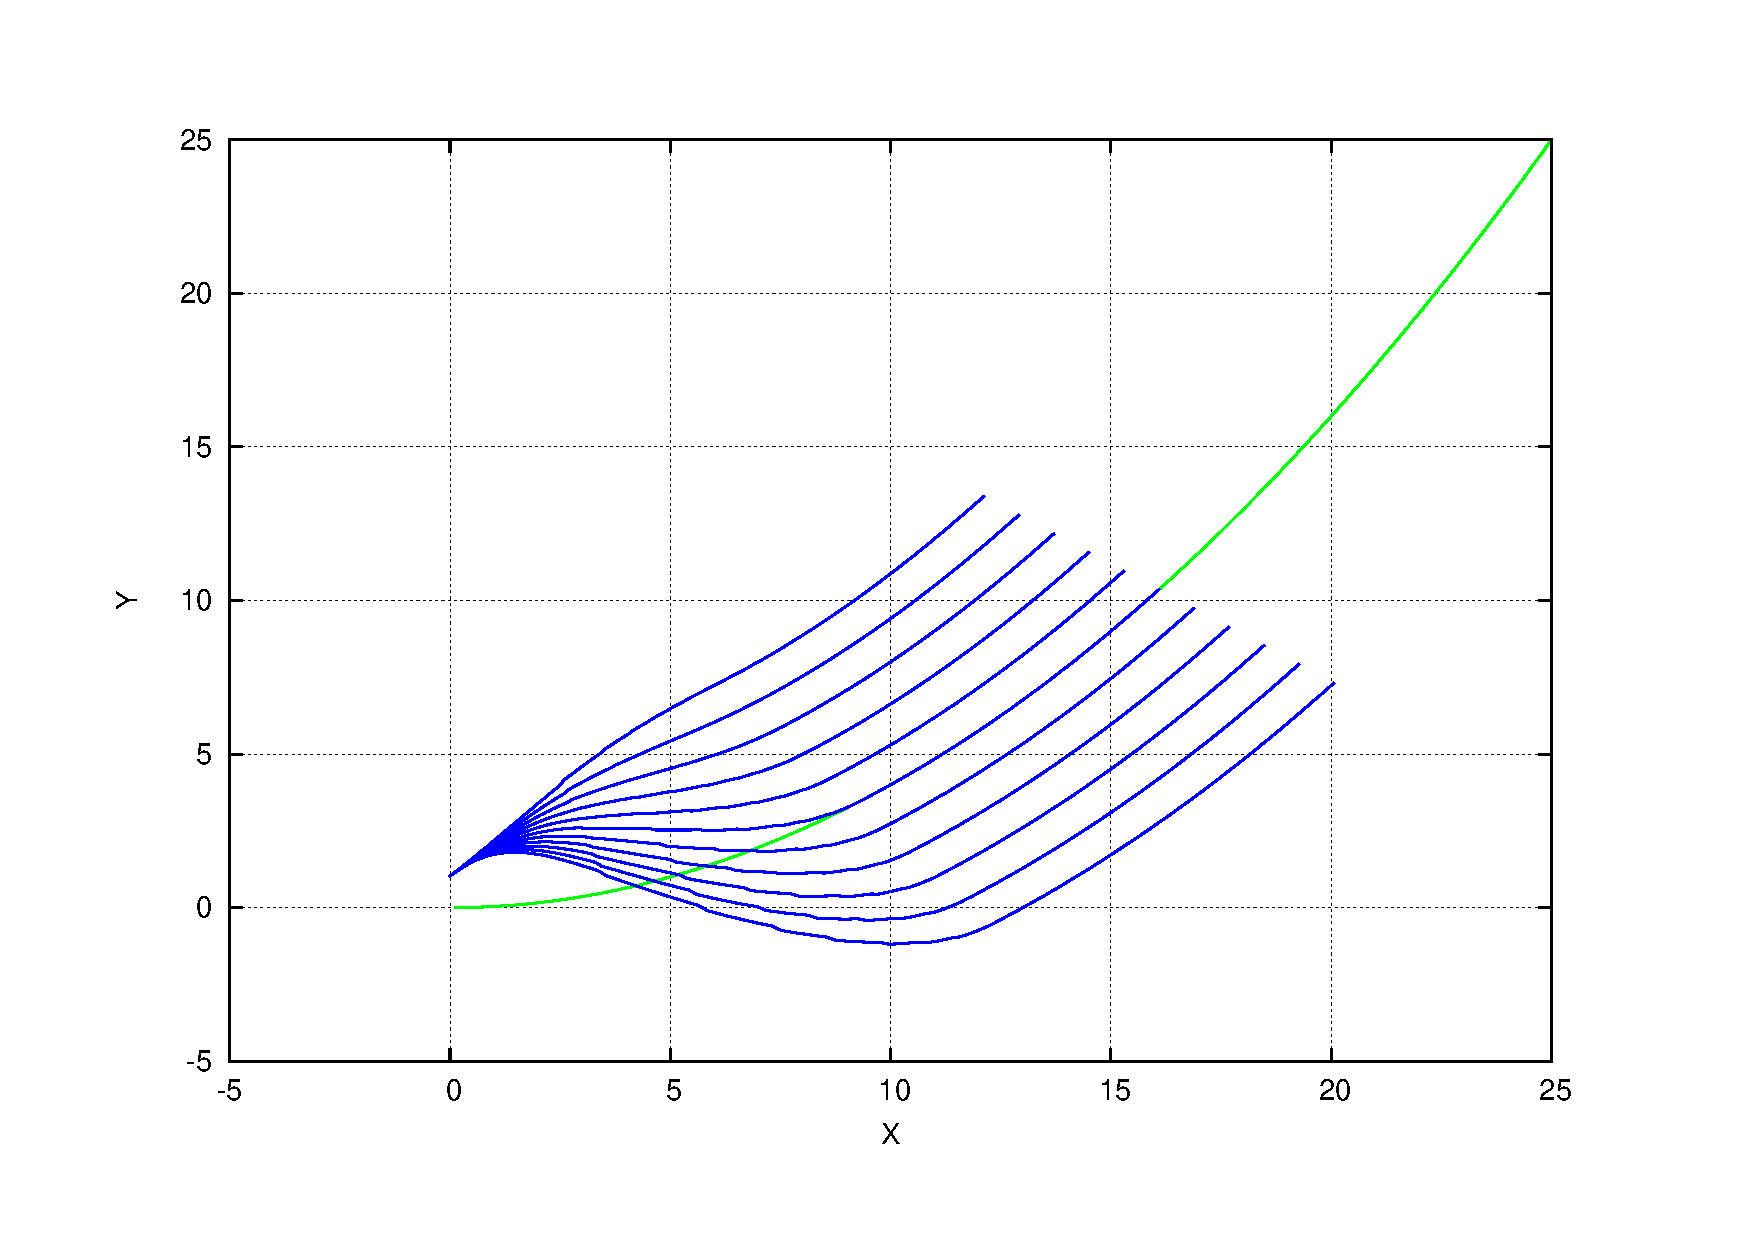
\includegraphics[width=\textwidth, trim=50 40 80 60,clip]{cartesian45}
    \caption{Euclidean space.}
    \label{fig:cp07_cartesian45}
    \end{subfigure}
\end{tabular}
\caption{Example in which the vehicle is rotated with respect to the path.}\label{fig:cp07_frenet45}
\end{figure}

Now the paths are in euclidean coordinates, we can evaluate which is the maximal distance they can reach individually if obstacles are considered. To do that, we iterate over the points in the trajectory, and check the cost associated to each cell $c_{ij}$ containing the point in the costmap computed in section \ref{ch:chapter07_01_01}. If this cost is over the value associated to the threshold $\tau_{circumscribed}$, the path is truncated at this point, as shown in figure \ref{fig:cp07_path_truncation}, where the generated paths are shown together with a color representation of the costmap, representing in blue the lower values, and in red the higher ones. Yellow and cyan correspond to cells in lethal and inscribed cells, respectively. The points iterated before reaching this cost will be kept, but it is very unlikely that this will be the winner path, as the occlusion cost will be maximal, and the length of the path shorter (see section \ref{ch:chapter07_01_04}). The reason for which we keep these points instead of removing completely the whole path is that, as the car will be traveling in crowded areas with many pedestrians, we want to keep moving even if we see that at this point each of the paths do not reach the maximal distance horizon until we enter in an unsafe cell. Obviously, in this case the speed is reduced according to the winner path length. However, if there is at least one path able to reach the last point in the tentative trajectory, this will be probably the winner one, thanks to the weights configuration described in the next section.

\begin{figure}[h!]
\centering
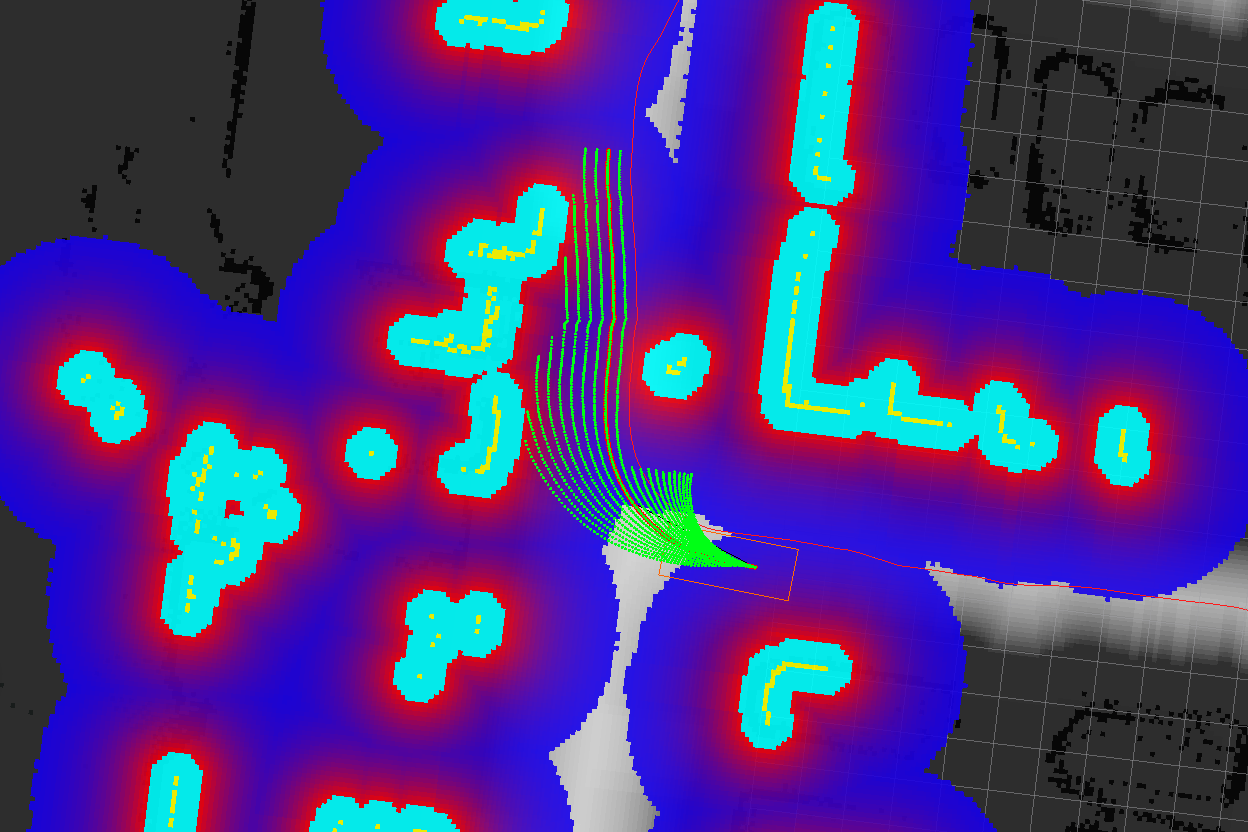
\includegraphics{example15}
\caption{Paths truncation example.}\label{fig:cp07_path_truncation}
\end{figure}

\subsection{Selection of the winner path}\label{ch:chapter07_01_04}

The winner path is selected among all the paths based on a cost function which is a linear combination of the values obtained from other cost functions scaled by their associated weighting factors. Occlusion, length, distance to the global path, curvature and consistency of the path is evaluated as follows:

\begin{equation}\label{eq:cp07_cost_function}
J[i] = \omega_o C_o[i] + \omega_l C_l[i] + \omega_d C_d[i] + \omega_{\kappa} C_{\kappa}[i] + \omega_c C_c[i]
\end{equation}

Here, $i$ is the path index, and $C_o$, $C_l$, $C_d$, $C_{\kappa}$ and $C_c$ are the costs of occlusion, length, distance to the global path, curvature and consistency, respectively. Their relatives $\omega_k$, $k \in \{o, l, d, \kappa, c\}$ are the associate weights that allow to adjust the influence of each of the costs to the final cost value. All these costs are normalized to $1.0$, and 

\begin{equation}\label{eq:cp07_weights_sum}
\sum_{{i \in \{o, l, d, \kappa, c\}}} w_i= 1.0
\end{equation}

, so it is easy to determine the proportional influence of each of the weights with respect to the others. Based on this, the value of $J[i]$ will be always inside the interval $[0\dots1]$.

The following costs will be computed for each candidate path independently from the euclidean space.

\paragraph{Occlusion}\label{ch:chapter07_01_04_00_01}

The occlusion cost is related to the safety of the path. This cost estimates the goodness of a path, being the bests paths those that pass far enough from the obstacles. To do that, we iterate along the path, simulating the footprint of the car at each position. The occlusion cost corresponding to the trajectory point $i$ will be the maximal cost of each of the cells $c_{ij} \in \mathcal{C}$ under the footprint of the car at that position. Based on this, the occlusion cost will be

\begin{equation}\label{eq:cp07_occlusion_cost}
C_o = {{max\{c_i\}} \over 255}, ~~~~~~ i=1 \dots L
\end{equation}

In this expression, $L$ is the length of the current path being evaluated. $max\{c_i\}$ is the maximal value of all the costs, associated to a point in the path. As we saw in section \ref{ch:chapter07_01_01}, the maximal value of each cost is $255$, so we divide the cost by this value, in order to normalize it to $1$.

\paragraph{Length}\label{ch:chapter07_01_04_00_02}

This costs represents the length of the current path. By iterating along the points in the path, we accumulate the distance between them, so we know the real distance traveled in euclidean coordinates. The longer that a path is, the better, as we assume that it means that paths are able to travel a longer distance. The expression that calculates this cost is:

\begin{equation}\label{eq:cp07_length_cost}
C_l = 1- {{\sum\limits_{i=1}^{L}\|p_i - p_{i - 1}\|} \over {q_{f_{max}} + s_f}}
\end{equation}

Here, $p_i$ is a certain point inside the evaluated path. $q_{f_{max}}$ is the maximal value that a $q_f$ can have for a certain path. Lengths are normalized to a value that a path will never reach. In our case, we decided that the sum of the maximal expected offset for $s$ and for $q$ is good enough (lengths will never trespass this value, while being small enough to allow an easy discrimination between paths). We subtract this cost from 1, in order to make it comparable to the rest of costs (lower values are preferred respect to the higher ones).

\paragraph{Distance to the global path}\label{ch:chapter07_01_04_00_03}

In our implementation, we included information about the average lateral offset respect to the global path. The use of this cost will help give the vehicle a trend to  come back to the global path after an occasional obstacle is avoided. This cost is computed as follows:

\begin{equation}\label{eq:cp07_lateral_cost}
C_d = {{\sum\limits_{i=1}^{L}\|p_i - nearest(p_i, g)\|} \over {L \cdot q_{f_{max}}}}
\end{equation}

, where $nearest(p, g)$ is the nearest point in the global path $g$ to the point $p$. This cost is normalized with respect to the maximal expected offset, $q_{f_{max}}$.

\paragraph{Curvature}\label{ch:chapter07_01_04_00_04}

This cost allows giving priority to the smoother paths. Let $p_(x_i, y_i), ~ i=1\cdots L$, be a point in the path. Then, 

\begin{equation}\label{eq:cp07_curvature_cost}
C_{\kappa} = max \left \{ {{x_i' \cdot y_i'' - x_i'' \cdot y_i'} \over {(x_i' + y_i')^{3/2}}} \right \}, ~~~~~~ i=1 \dots L
\end{equation}

\paragraph{Consistency}\label{ch:chapter07_01_04_00_05}

This cost avoids the continuous changes in the winner paths between iterations. Once the vehicle starts a maneuver, the idea is keeping this behavior in the following iterations.

This is done through the following expression:

\begin{equation}\label{eq:cp07_consistency_cost}
C_c = {1 \over {s_2 - s_1}} \int \limits_{s_1}^{s_2} l_i ~ ds
\end{equation}

This equation is better understood if we look at figure \ref{fig:cp07_consistency_cost}. There, the lateral cost $l_i(s)$ is the distance between the current and the previous winner path at the same longitudinal position $s$; $s_1$ and $s_2$ are the first and last positions over $s$ for which there are points in common in both trajectories.

\begin{figure}[h!]
  \centering
  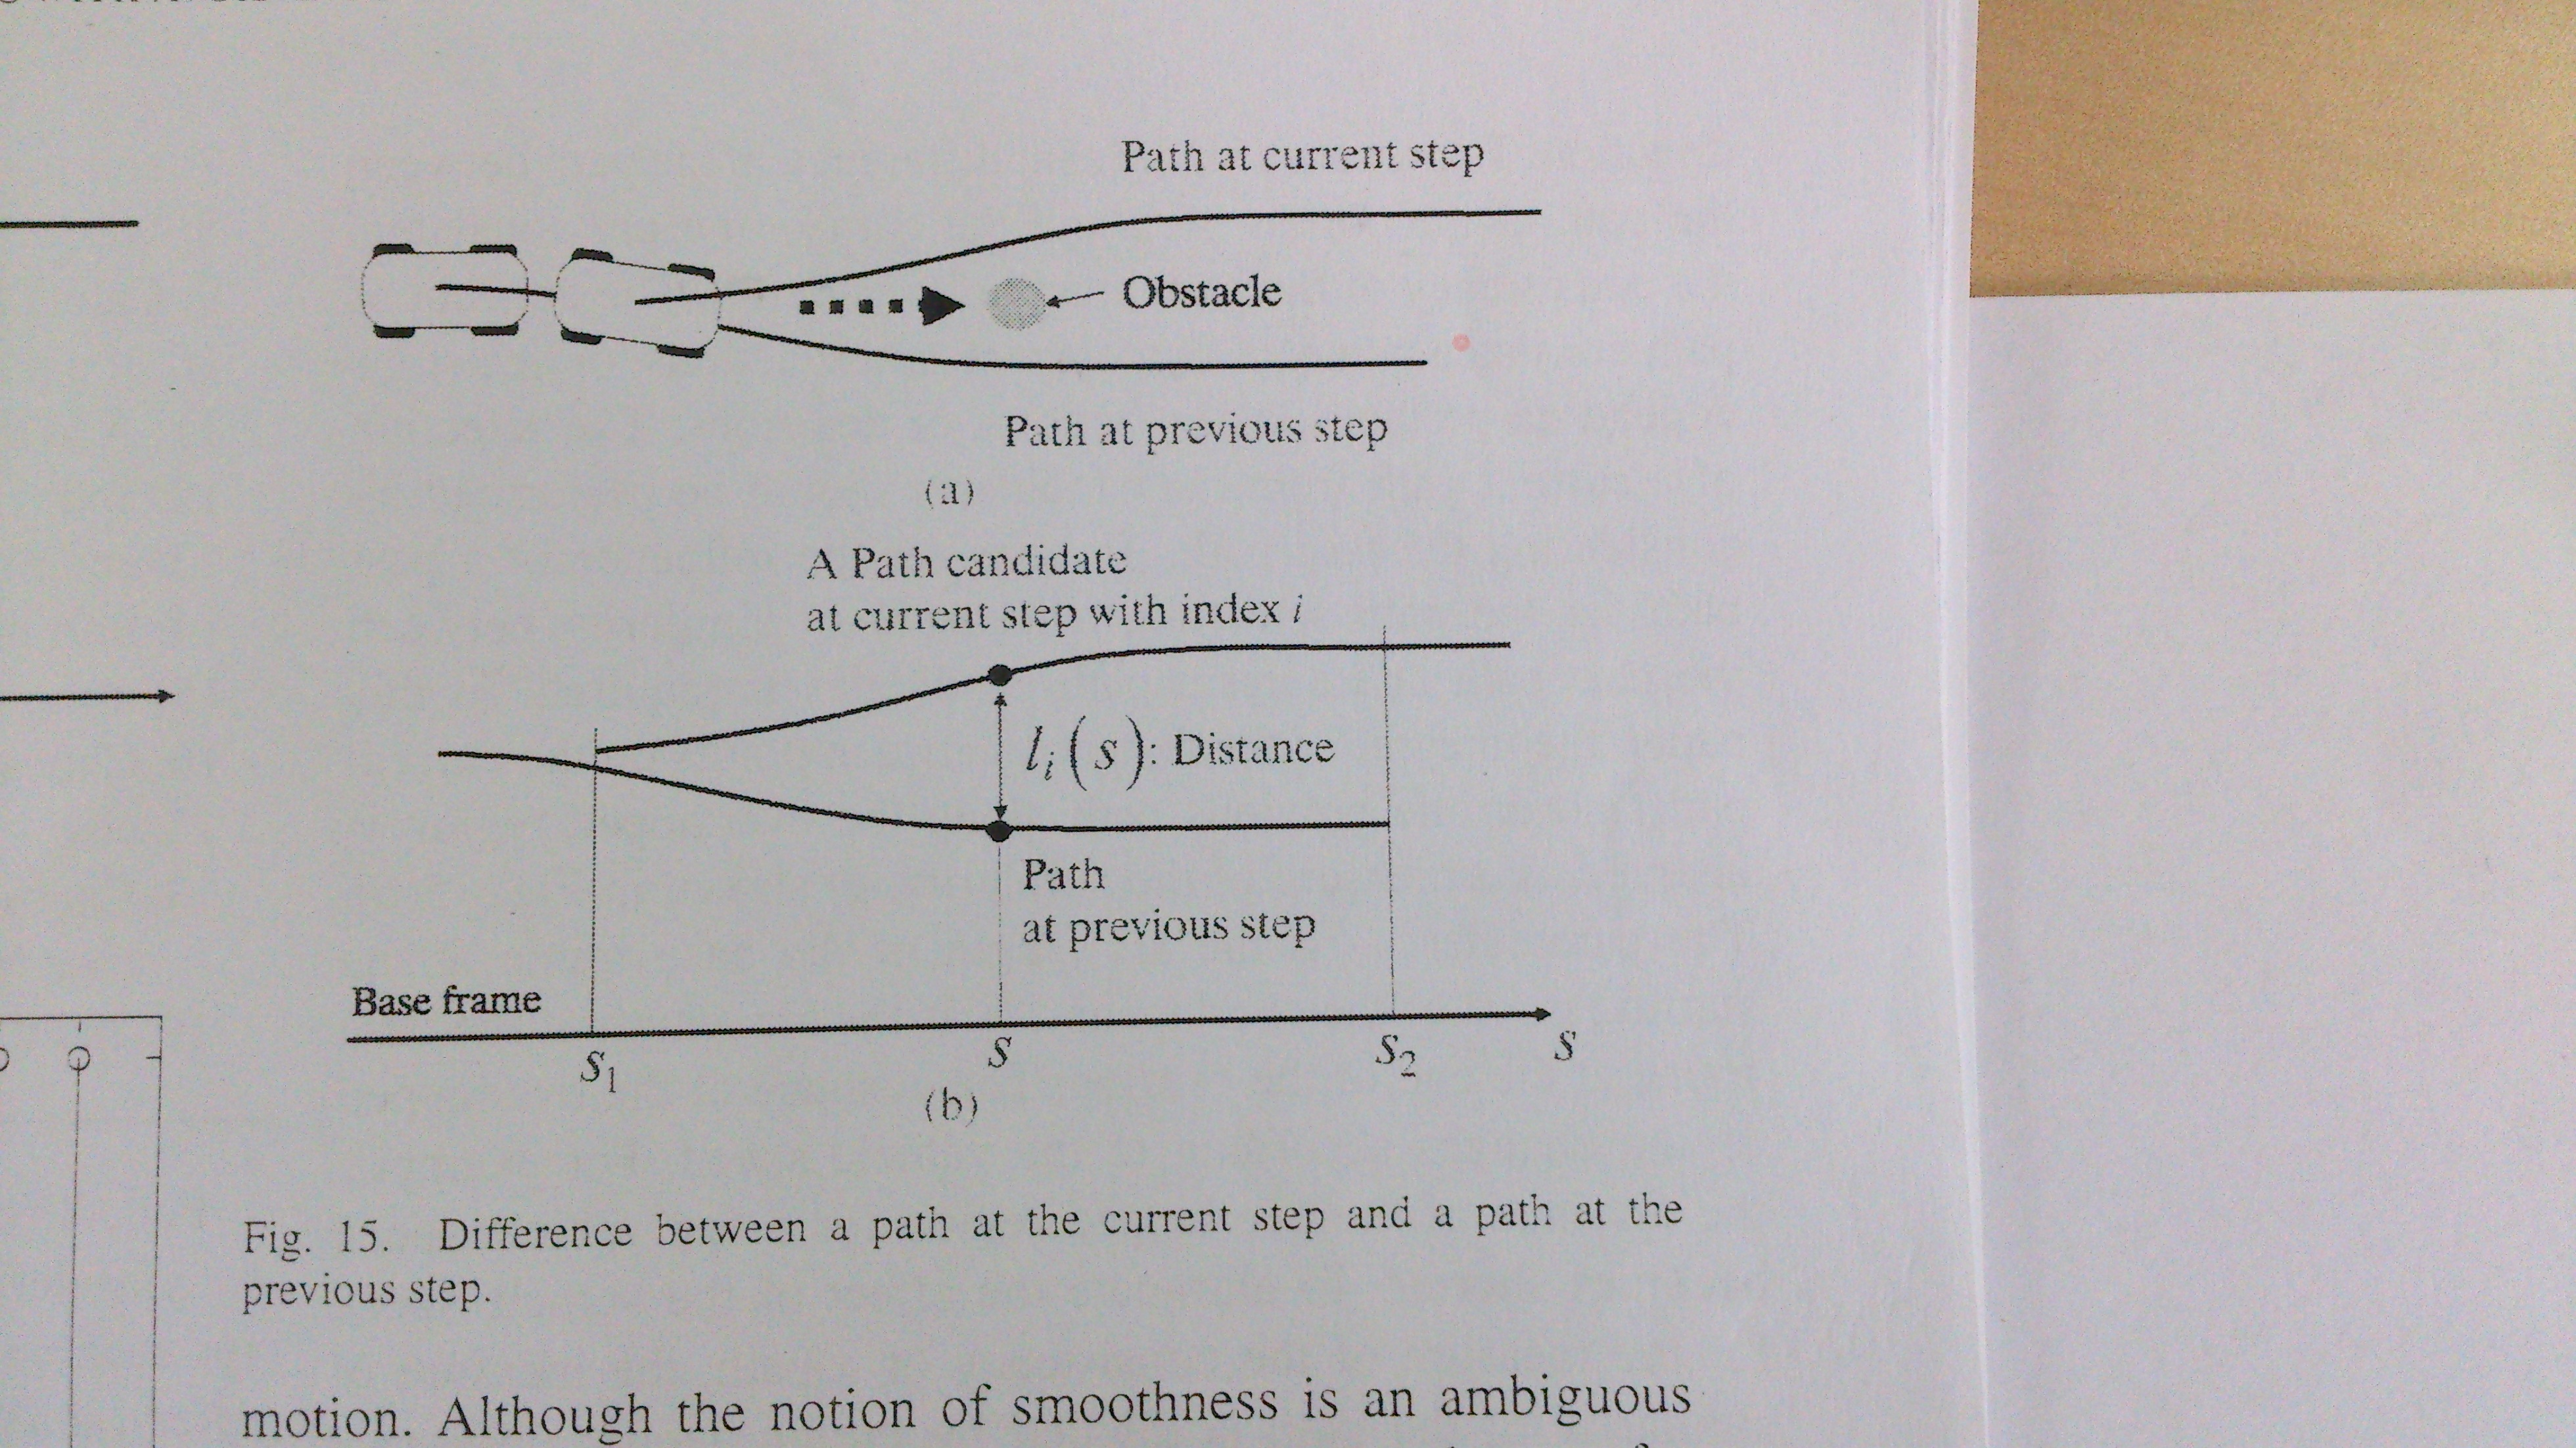
\includegraphics[width=\textwidth]{consistency_cost}
  \caption{Representation of the way in which the consistency cost is computed.}\label{fig:cp07_consistency_cost}
\end{figure}

\subsubsection{Selection of the winner path}\label{ch:chapter07_01_04_01}

Once all the costs are computed, we just apply the expression described in equation \ref{eq:cp07_cost_function}. In those paths for which it is impossible to advance due to the presence of a nearby obstacle because the car is bad oriented to the global path (meaning that no valid paths can be generated in this situation), the cost will be negative (invalid path).

From all the paths, we select that with the smallest cost, which will be the winner path $W$. If all paths are set as invalid, the car cannot advance. If the reason for that situation is the presence of a nearby obstacle, the vehicle waits until the way is clearer. If this situation does not change for a long time, a new global plan is computed.

If no valid paths were found because the vehicle has a bad orientation respect to the global plan, a recovery behavior process is started.

\subsection{Computation of the vehicle commands}\label{ch:chapter07_01_04}

The last step required in order to follow the trajectory obtained from the global planner is the computation of the steering angle and speed commands that will be sent to the built-in controller of the vehicle. The way in which this is done is quite simple. Over the winner path, we apply a \ac{PID} controller in which we try to minimize the distance and heading of the vehicle respect to that trajectory. Using this controller and a model of the vehicle, we can compute the proper values, which are finally sent to the vehicle.

\subsection{Recovery behavior}\label{ch:chapter07_01_05}

When the lateral offset of a path is bigger than the radius of curvature of base frame, paths can not be generated using the approach described before. Because of that, we propose to compute the paths in a different way, so the vehicle can advance towards the global plan until this restriction is satisfied again. The way in which we do that is through the use of a model of the behavior of the vehicle. This model is the same Ackerman model used in \cite{espelosin2013path}.

Four paths are evolved in a parameterized time $t$, considering a low speed. Two of these paths are generated considering a positive speed (forward movement) and the top left and top right steering position, and the other two are similar, but using a negative speed. All these four paths are weighted following the same process described in in \ref{ch:chapter07_01_04}, and the winner is selected. The resulting speed and steering commands for the recovery behavior process will be those used to evolve the winner path.

% \section{Putting all together}\label{ch:chapter08_07}
% \comment{No tengo muy claro si esto debería ir aquí o en las conclusiones}
% 
% Using the methods described in this thesis, we are now able to detect the obstacles existing in the environment and track them along the frames. Also, we are able to generate trajectories that can be followed by our vehicle in order to reach a certain point, and we know how to compute the commands that the vehicle need to follow these trajectories. Now it is time to put everything together.
% 
% In the images shown at figure \ref{fig:cp07_whole_pipeline}, we can see an integration of some of the methods described in this thesis. These images have been extracted from the videos available at \url{http://youtu.be/08mAOD6bT9w} (for the Stixels based example); and \url{http://youtu.be/SCQ6_GYjbJs} and \url{http://youtu.be/rn4iIafBFZc} (for the Particle Filter based one). In these methods, we have included the obstacles detected using the methods described in chapters \ref{ch:chapter04} and \ref{ch:chapter05}, which are incorporated to the costmap described in section \ref{ch:chapter07_01_01}. Unfortunately, at this time the described implementation of the costmap do not accept temporal information, so we just can include the detected obstacles, but not the information about their future movement that could be obtained thanks to the tracks detected. Also, as we said before, the global planner described in section \ref{ch:chapter06} was discarded as it is not longer needed in this form, but we think on it as a solution for the fast generation of \acp{RNDF}.
% 
% \begin{figure*}[h!]
%   \begin{subfigure}[b]{\textwidth}
%     \centering
%     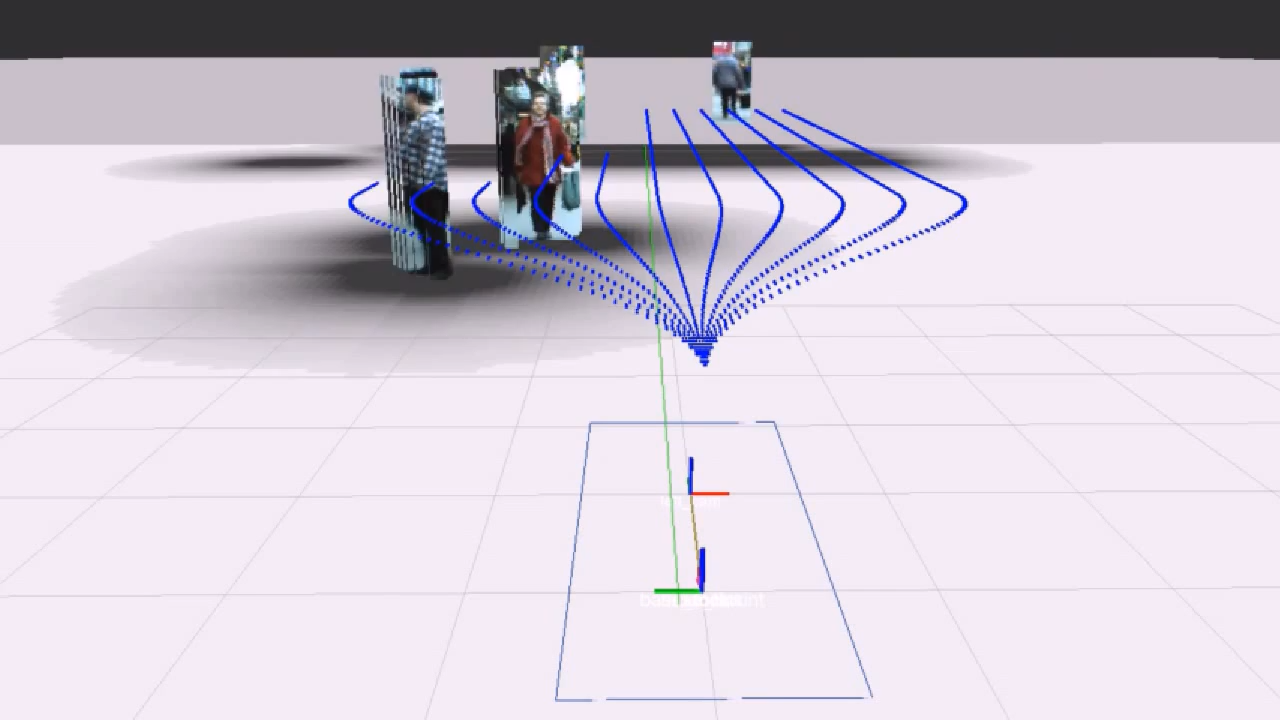
\includegraphics[width=\textwidth, height=0.75\textwidth]{stixels_whole_pipeline}
%     \caption{Integration of the whole pipeline of the application, including the stixel based method, described in chapter \ref{ch:chapter04}.}\label{fig:cp07_stixels_whole_pipeline}
%   \end{subfigure}
%   ~
%   \begin{subfigure}[b]{\textwidth}
%     \centering
%     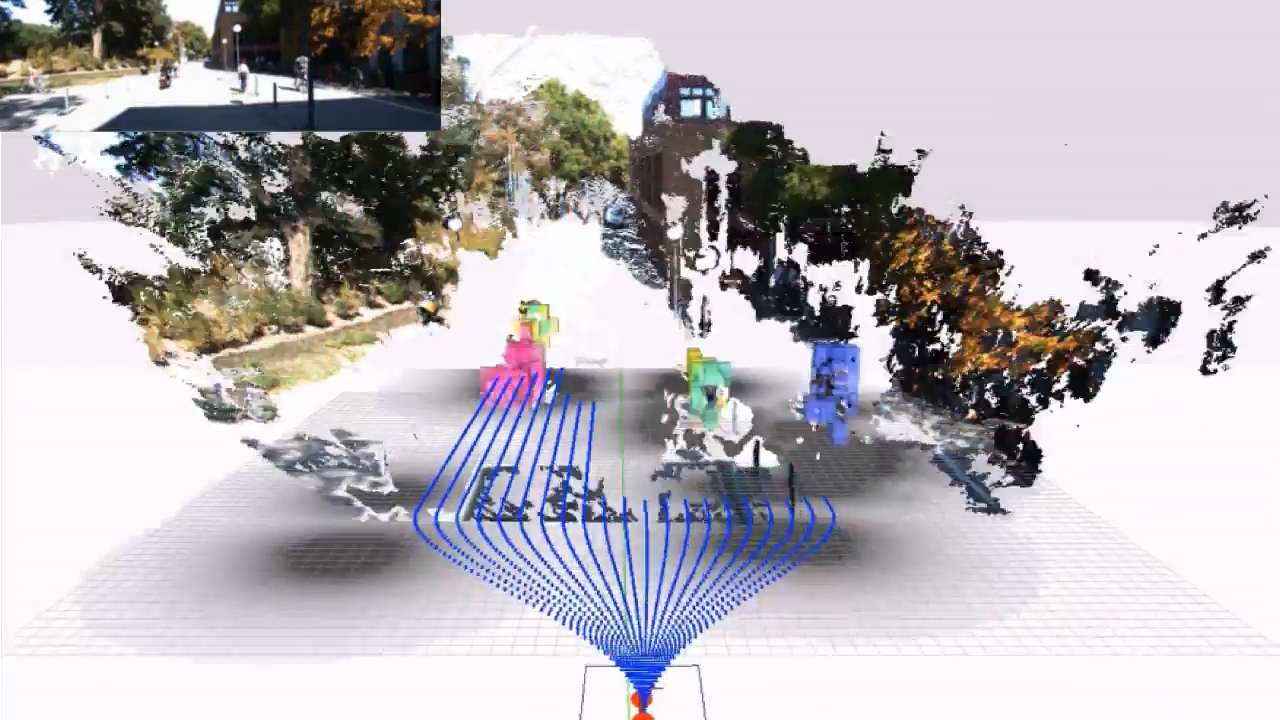
\includegraphics[width=\textwidth, height=0.75\textwidth]{particle_filter_whole_pipeline}
%     \caption{Integration of the whole pipeline of the application, including the particle filter based method, described in chapter \ref{ch:chapter05}.}\label{fig:cp07_particle_filter_whole_pipeline}
%   \end{subfigure}
%   \caption{Integration of the full pipeline of the application described in this thesis. Frames have been extracted from the videos available at \url{http://youtu.be/08mAOD6bT9w}, \url{http://youtu.be/SCQ6_GYjbJs} and \url{http://youtu.be/rn4iIafBFZc}.}\label{fig:cp07_whole_pipeline}
% \end{figure*}
% 
% Anyway, the integration of the method with the planner described in this chapter is quite good. We can see in both images that the planner reacts properly to the objects detected and that, given a pair images, both methods are able to detect the obstacles, allowing a safe trip. In general, both methods are suitable for the evaluated scenarios, being the most limiting features those inherent to the methods, which were described in chapters \ref{ch:chapter04} and \ref{ch:chapter05}.

\section{Summary}\label{ch:chapter07_04}

In this chapter, we have seen a method able to follow efficiently a given trajectory, while avoiding the potential obstacles in the way. The use of a curvilinear coordinate system for the generation of a set of candidate trajectories simplifies the calculations while allows creating soft paths that makes the vehicle to converge to the followed track in a way as smooth as possible. Moreover, these paths are generated with different lateral offsets regarding to the global plan, so we are able to avoid an obstacle even if it is in the middle of the path. Finally, as speed is out the model used for the generation of the tracks, it is reduced to the computation of a set of parameters that define a third order polynomial. Speed and steering angle are then computed, using a \ac{PID} controller over the winner path, which is chosen based on a cost function.

There are some videos in which the good behavior of this method is available, as those in \url{http://verdino.webs.ull.es/node/109}, \url{http://verdino.webs.ull.es/node/103}, \url{http://verdino.webs.ull.es/node/105} and \url{http://verdino.webs.ull.es/node/102}; and an early version of the method in \url{http://verdino.webs.ull.es/node/108}. Also, the videos introduced in section \ref{ch:chapter07_03}, available at \url{http://youtu.be/08mAOD6bT9w}, \url{http://youtu.be/rn4iIafBFZc} and \url{http://youtu.be/SCQ6_GYjbJs}, show how the integration of the method with the algorithm described in chapters \ref{ch:chapter04} and \ref{ch:chapter05} is possible. Finally, in the future, the code related to this part will be available at \url{https://github.com/ull-isaatc/grull_ackermann_base_local_planner}. \comment{¿Tiene sentido poner el vídeo de la versión anterior? (Es que da bastante el pego). ¿Tiene sentido poner la url de dónde estará el código si ni siquiera está claro que lo vayamos a liberar algún día?}

As future work, we can study the inclusion of new costs or long-term control strategies, as those used in \cite{werling2010optimal}. Furthermore, the computation of the steering angle based on the winner path could be improved through the use of a predictive controller.

In the next chapter, we will see the results obtained for all the methods described until now, which will be give us a clear idea of their performance, and the advantages and disadvantages of using such methods.


